% !TEX program = xelatex
% ============================================================================
%  从 3D 高斯到三角网格：SuGaR 复现与深度-法向一致性正则改动
%  本文件由 outputs/reports/report.docx 自动转换生成（scripts 见 README_LATEX.md）
%  编译方式：XeLaTeX（Overleaf 中在 Menu -> Compiler 选择 XeLaTeX）
% ============================================================================
\documentclass[UTF8,a4paper,11pt]{ctexart}

\usepackage{geometry}
\geometry{left=2.5cm,right=2.5cm,top=2.5cm,bottom=2.5cm}
\usepackage{graphicx}
\usepackage{booktabs}
\usepackage{longtable}
\usepackage{array}
\usepackage{caption}
\usepackage{amsmath}
\usepackage{xcolor}
\usepackage{float}
\usepackage[hidelinks]{hyperref}

% verbatim 代码块里出现的希腊字母（如 λ）交给 CJK 字体排版，避免等宽字体缺字
\makeatletter
\@ifpackageloaded{xeCJK}{\xeCJKDeclareCharClass{CJK}{"03B1,"03B2,"03BB,"03C3,"03BC,"0394}}{}
\makeatother

\graphicspath{{figures/}}
\captionsetup{font=small,labelsep=quad}
\captionsetup[figure]{name=图}
\captionsetup[table]{name=表}
\setlength{\parskip}{0.5em}
\renewcommand{\arraystretch}{1.15}
\setcounter{secnumdepth}{0}   % 章节号已写在标题文字里，避免重复编号

\begin{document}

\begin{center}
{\LARGE\bfseries
从 3D 高斯到三角网格：SuGaR 复现\\
与深度-法向一致性正则改动}
\end{center}
\vspace{4pt}
浙江大学博士代码考核 ｜ 6 小时限时复现与魔改 ｜ 全中文技术报告

\textbf{目标开源项目：}SuGaR（CVPR 2024），官方 commit 7c10c4a

\textbf{数据集与场景：}Tanks \& Temples / Truck（3DGS 官方打包 tandt\_db.zip，含 COLMAP 稀疏重建）

\textbf{改动点：}① 训练端：在 coarse SuGaR 训练主循环中加入深度-法向一致性正则 L\_DNC（借鉴 2DGS 思路，自行实现）；② 提取端：把泊松重建深度改为按场景尺度自动推算（移植自 Frosting）；③ 提取端扩展（A100）：q=0 清洗 + M2-B DBSCAN 剪枝 + M1+a 背景 Poisson 深度，碎片 $-$43\%，渲染指标不变

\textbf{对照组：}训练端五组完整重跑：$\lambda$=0 / 0.05 / 0.2 / 0.2+detach 诊断 / 官方 dn\_consistency；提取端在同一个 $\lambda$=0 模型上扫 Poisson 深度与顶点密度分位

\textbf{报告生成时间：}2026 年 09 月 13 日 10:43

\begin{center}
\fbox{\parbox{0.94\linewidth}{\small
\textbf{数据来源声明}\\[2pt]
本报告中出现的全部实验数值均由脚本从 outputs/metrics/summary.csv 及 outputs/metrics/ 下的 render\_*.json、geometry\_*.json、各 run 的 train\_stats.json 与 dnc\_log.csv 自动读取并排版，未经人工转录；未跑出结果的位置显示“未完成”，不做任何估计或补值。\\[2pt]
CUDA 光栅化（diff-gaussian-rasterization）的原子累加本身非确定，即使固定 seed=0，逐次运行也会有微小数值差异，本报告中的指标据此理解。
}}
\end{center}
\section{摘要}
本报告完成了 SuGaR（Surface-Aligned Gaussian Splatting）从 3D 高斯到三角网格的完整短流水线复现：3D Gaussian Splatting 训练 7000 迭代 $\rightarrow$ coarse SuGaR 密度正则训练至 15000 迭代 $\rightarrow$ 泊松表面重建导出三角网格，并在此基础上做了一处进入训练主循环的改动：深度-法向一致性正则（Depth-Normal Consistency，下称 DNC）。改动思路借鉴 2D Gaussian Splatting（SIGGRAPH 2024）提出的 depth-normal consistency 损失，将其移植到 SuGaR 的三维椭球表示上，并针对法向符号歧义、低不透明度像素与物体边缘设计了掩码。实验在 Tanks \& Temples 的 Truck 场景上以 $\lambda$ $\in$ \{0, 0.05, 0.2\} 做三组完整对照，统一评测渲染质量（PSNR / SSIM / LPIPS）与网格几何（稀疏点到网格距离、拓扑碎片、法向平滑度）。

本工作在 Tanks\&Temples Truck 场景上完整复现了 3DGS(7k) $\rightarrow$ coarse SuGaR(15k, density 正则) $\rightarrow$ Poisson 网格提取的短流程，并在 coarse 训练主循环中加入像素级的深度-法向一致性正则（DNC）。对照实验（$\lambda$=0 / 0.05 / 0.2，各一次完整重跑）表明：在 7k$\rightarrow$15k 的短预算下，DNC \textbf{没有}带来几何改善，反而随 $\lambda$ 增大单调损害渲染与几何；$\lambda$=0.2 时场景坍缩为大尺度半透明薄片。进一步的诊断实验（切断损失对深度的梯度）把 PSNR 从 13.24 dB 恢复到 24.40 dB（$\lambda$=0 为 24.62 dB），证实退化源于"抹平渲染深度"这一平凡解，但几何指标仍未优于基线。本报告如实报告这一负结果与其机理，在写作后期核实到官方仓库已内置同类正则（dn\_consistency）并将其作为对照组：官方实现在同样 $\lambda$=0.05 下碎片分量 $-$16\%、二面角均值 $-$10\%、PSNR 仅 $-$0.24 dB。因此结论修正为：深度-法向一致性这一思路在 SuGaR coarse 阶段有效，本工作独立实现的版本因实现细节差异而失效；本报告如实给出负结果、退化机理与两版实现的差异清单。

与训练端结果的统一解读：训练端的官方 dn\_consistency 用 PSNR $-$0.24 dB 换碎片 $-$16\%；提取端改动零渲染代价换碎片 $-$43\%，两者作用在流水线的不同阶段、相互正交，可以叠加；PSNR 不变不是"没提升"，而是该指标测不到提取阶段。本节全部数字来自 results\_a100/metrics/summary.csv 与对应 JSON，该机器已用自写 union-find 与边表独立复算了分量数、碎片数与边界边（与其评测脚本逐位一致）。

\subsection{预注册的可检验假设}
\textbf{H1（几何）：}$\lambda$>0 时，网格碎片连通分量数下降、COLMAP 稀疏点到网格距离中位数下降、网格法向更平滑。

\textbf{H2（渲染代价）：}测试视角 PSNR 变化在 $\pm$0.5 dB 以内；若下降更多，如实报告为代价。

\textbf{H3（叠加关系）：}DNC 与 SuGaR 原有的 SDF 法向损失不冲突，训练中两者同时下降。

\begin{itemize}
\setlength{\itemsep}{2pt}
  \item H1（几何改善）：\textbf{不支持}。$\lambda$=0.05 时碎片分量 2137$\rightarrow$2324、稀疏点到网格距离中位数 0.0687\%$\rightarrow$0.1421\%（相对相机尺度）、二面角均值上升；$\lambda$=0.2 的碎片数下降到 1177 是网格整体坍缩（面数 370k$\rightarrow$223k，包围盒从 $\pm$23 缩到 $\pm$9.7）的副产物，不构成证据；detach 组碎片 2142、距离中位数 0.0839\%，仍不优于 $\lambda$=0。
  \item H2（渲染代价 $\pm$0.5 dB 内）：\textbf{不支持}。$\lambda$=0.05 为 $-$2.17 dB，$\lambda$=0.2 为 $-$11.38 dB。仅 detach 变体满足（$-$0.22 dB）。
  \item H3（与原有 SDF 法向损失不冲突）：\textbf{仅在"两者同时下降"的操作性定义下成立}；两组 $\lambda$ 的 L\_dnc 与 sdf\_better\_normal\_loss 均单调下降，但几何并未变好，说明"损失下降"与"表面质量"在此脱钩，H3 的定义本身不足以作为质量判据。
\end{itemize}
\section{1 环境与数据}
\subsection{1.1 运行环境}
{
\begin{longtable}{>{\raggedright\arraybackslash}p{5.18cm}>{\raggedright\arraybackslash}p{9.86cm}}
\caption{运行环境与关键依赖版本}\label{tab:1}\\
\toprule
\textbf{项} & \textbf{值} \\
\midrule
\endfirsthead
\multicolumn{2}{l}{\footnotesize（续表 1）}\\
\toprule
\textbf{项} & \textbf{值} \\
\midrule
\endhead
\bottomrule
\endlastfoot
操作系统 & Ubuntu 22.04.3 LTS \\
GPU & 2 $\times$ NVIDIA H200（143771 MiB / 卡，驱动 575.57.08） \\
python & 3.10.12 (main, Jan  8 2026, 06:52:19) [GCC 11.4.0] \\
venv & /scratch/e1351071/virtualenvs/zju\_test \\
torch & 2.4.1+cu121 \\
torchvision & 0.19.1+cu121 \\
torch.version.cuda & 12.1 \\
cuda available & True | device count: 2 \\
GLIBCXX\_USE\_CXX11\_ABI & False \\
matplotlib & 3.10.9 \\
numpy & 1.26.4 \\
open3d & 0.19.0 \\
opencv-python & 4.11.0.86 \\
plyfile & 1.1.3 \\
pytorch3d & 0.7.8 \\
scikit-learn & 1.7.2 \\
scipy & 1.15.3 \\
simple-knn & 0.0.0 \\
commit & 7c10c4ae4a267dece512f5c7f40ed212a0a2ab44 \\
系统 nvcc & 12.1 \\
\end{longtable}
}
来源：notes/ENV.md（由 scripts/gen\_env\_md.sh 自动抓取），完整冻结清单见 notes/pip\_freeze.txt。

\subsection{1.2 数据集与划分}
{
\begin{longtable}{>{\raggedright\arraybackslash}p{4.10cm}>{\raggedright\arraybackslash}p{10.94cm}}
\caption{数据集、分辨率与训练/测试划分}\label{tab:2}\\
\toprule
\textbf{项} & \textbf{值} \\
\midrule
\endfirsthead
\multicolumn{2}{l}{\footnotesize（续表 2）}\\
\toprule
\textbf{项} & \textbf{值} \\
\midrule
\endhead
\bottomrule
\endlastfoot
数据来源 & 3DGS 官方发布包 tandt\_db.zip（含 Tanks \& Temples 与 Deep Blending） \\
使用场景 & data/tandt/truck（含 COLMAP sparse/0 稀疏重建） \\
图像总数 & 251 张 \\
渲染分辨率 & 979 $\times$ 546 像素 \\
训练 / 测试划分 & llffhold=8（按文件名排序后索引 \% 8 == 0 为测试）$\rightarrow$ 训练 219 张 / 测试 32 张 \\
几何参考 & COLMAP 稀疏点（track 长度 $\ge$ 3 且落在前景包围盒内），参考点数 88,066 个 \\
\end{longtable}
}
所有 run（含 3DGS、三组 coarse SuGaR 与网格提取）使用完全相同的划分与相机。

\section{2 复现流程与命令}
完整流水线分三步，三组对照共用同一个 3DGS 检查点以保证公平：

\begin{itemize}
\setlength{\itemsep}{2pt}
  \item 第一步：3D Gaussian Splatting 训练 7000 迭代，产出 point\_cloud/iteration\_7000/point\_cloud.ply；
  \item 第二步：coarse SuGaR（density 正则模式）从该检查点续训到 15000 迭代，其中 7000--9000 为熵正则阶段，9000 迭代做一次 opacity<0.5 的硬剪枝，9000 起进入 SDF 正则；
  \item 第三步：extract\_mesh.py 以 surface\_level=0.3、decimation 目标 200000 做泊松重建与抽取。
\end{itemize}
关于 decimation 语义的勘误：命令行 -d 200000 并非“输出 20 万面”，而是对前景网格与背景网格各自抽取到 20 万个三角形的目标，两者合并后总面数约为 37 万，属正常现象。三组使用完全相同的参数。

\textbf{第一步（3DGS 7000 迭代）的实际命令：}

{\small
\begin{verbatim}
cd $PROJ_ROOT/repo/SuGaR
CUDA_VISIBLE_DEVICES=0 python gaussian_splatting/train.py \
  -s $PROJ_ROOT/data/tandt/truck \
  -m $PROJ_ROOT/outputs/baseline/gs_truck \
  --iterations 7000 --save_iterations 7000 --test_iterations 7000 --eval
\end{verbatim}
}
\textbf{第二、三步（三组 coarse 训练 + 网格提取）的实际命令：}

{\scriptsize
\begin{verbatim}
cd /scratch/e1351071/zju_test/repo/SuGaR_dev

# --- coarse_base_seed0 (GPU0, λ=0) ---
python train_coarse_density.py \
  -s /scratch/e1351071/zju_test/data/tandt/truck \
  -c /scratch/e1351071/zju_test/outputs/baseline/gs_truck/ \
  -i 7000 -o /scratch/e1351071/zju_test/outputs/runs/coarse_base_seed0 \
  --eval True --gpu 0 --seed 0 --dnc_factor 0 --dnc_start 9000
python extract_mesh.py \
  -s /scratch/e1351071/zju_test/data/tandt/truck \
  -c /scratch/e1351071/zju_test/outputs/baseline/gs_truck/ -i 7000 \
  -m /scratch/e1351071/zju_test/outputs/runs/coarse_base_seed0/sugarcoarse_3Dgs7000_densityestim02_sdfnorm02/15000.pt \
  -l 0.3 -d 200000 --eval True --gpu 0 \
  -o /scratch/e1351071/zju_test/outputs/runs/mesh_base_seed0

# --- coarse_dnc005 (GPU1, λ=0.05) ---
python train_coarse_density.py \
  -s /scratch/e1351071/zju_test/data/tandt/truck \
  -c /scratch/e1351071/zju_test/outputs/baseline/gs_truck/ \
  -i 7000 -o /scratch/e1351071/zju_test/outputs/runs/coarse_dnc005 \
  --eval True --gpu 1 --seed 0 --dnc_factor 0.05 --dnc_start 9000
python extract_mesh.py \
  -s /scratch/e1351071/zju_test/data/tandt/truck \
  -c /scratch/e1351071/zju_test/outputs/baseline/gs_truck/ -i 7000 \
  -m /scratch/e1351071/zju_test/outputs/runs/coarse_dnc005/sugarcoarse_3Dgs7000_densityestim02_sdfnorm02/15000.pt \
  -l 0.3 -d 200000 --eval True --gpu 1 \
  -o /scratch/e1351071/zju_test/outputs/runs/mesh_dnc005

# --- coarse_dnc02 (GPU1, λ=0.2) ---
python train_coarse_density.py \
  -s /scratch/e1351071/zju_test/data/tandt/truck \
  -c /scratch/e1351071/zju_test/outputs/baseline/gs_truck/ \
  -i 7000 -o /scratch/e1351071/zju_test/outputs/runs/coarse_dnc02 \
  --eval True --gpu 1 --seed 0 --dnc_factor 0.2 --dnc_start 9000
python extract_mesh.py \
  -s /scratch/e1351071/zju_test/data/tandt/truck \
  -c /scratch/e1351071/zju_test/outputs/baseline/gs_truck/ -i 7000 \
  -m /scratch/e1351071/zju_test/outputs/runs/coarse_dnc02/sugarcoarse_3Dgs7000_densityestim02_sdfnorm02/15000.pt \
  -l 0.3 -d 200000 --eval True --gpu 1 \
  -o /scratch/e1351071/zju_test/outputs/runs/mesh_dnc02
\end{verbatim}
}
以上命令原样摘自 notes/RUNLOG.md 与 notes/RUNLOG\_s34.md，未做改写；完整命令另见附录 A。

随机性控制：3DGS 的 safe\_state() 固定 random / numpy / torch 的 seed 为 0；三组 coarse 训练显式传入 --seed 0。但 CUDA 光栅化的原子累加本身非确定，因此逐次运行仍会有微小数值差异，本报告不把 0.01 dB 量级的差异当作显著差异。

\section{3 改动动机与实现}
本工作一共做了两处进入主流程的改动：训练端的深度-法向一致性正则（本章，是主要改动），以及提取端的自动泊松深度（移植自 Frosting，见 5.4 节）。两者互不依赖，可以单独开关。

\subsection{3.1 动机}
SuGaR 用 SDF / density 正则把高斯压扁并贴到表面上，但每个高斯的法向只受到采样点级别的 SDF 约束，相邻高斯之间的法向可以互相不一致。泊松重建以表面采样点及其法向为输入，法向噪声会直接转化为网格褶皱与漂浮碎片。DNC 的想法是：既然渲染深度图本身就编码了几何，那么由深度图差分得到的几何法向 N\_d 与渲染出的高斯法向 N 应当一致；在像素尺度上强制两者一致，等价于要求相邻高斯共面。

\subsection{3.2 思路来源与自己的贡献}
思路来源：2D Gaussian Splatting（SIGGRAPH 2024，文献 [3]）提出的 depth-normal consistency 损失。本工作把它移植到 SuGaR 的 coarse 阶段，属于借鉴已发表思路并自行实现，未复制 2DGS 的任何代码。相对原思路，本实现需要额外处理三件事：

\begin{itemize}
\setlength{\itemsep}{2pt}
  \item P1 表示差异：2DGS 的基元是二维圆盘，法向是其固有属性；SuGaR 的基元是三维椭球，法向取最短 scale 轴经四元数旋转后的方向，且存在正负两个朝向，需要按相机方向翻转并在损失中取绝对值；
  \item P2 与原有损失的叠加关系：SuGaR 已有采样点级别的 SDF 法向损失，DNC 是像素级、跨高斯的约束，两者是否冗余或冲突需要用实验回答（对应假设 H3，见图中训练曲线）；
  \item P3 掩码设计：渲染法向图是 $\alpha$ 合成的结果，低不透明度像素会得到接近零向量、方向无意义的法向，因此在计划原有的三条掩码之外增加了 $\|$N\_raw$\|$ > 0.1 的数值保护条件。
\end{itemize}
\subsection{3.3 损失定义}
\begin{figure}[H]
\centering
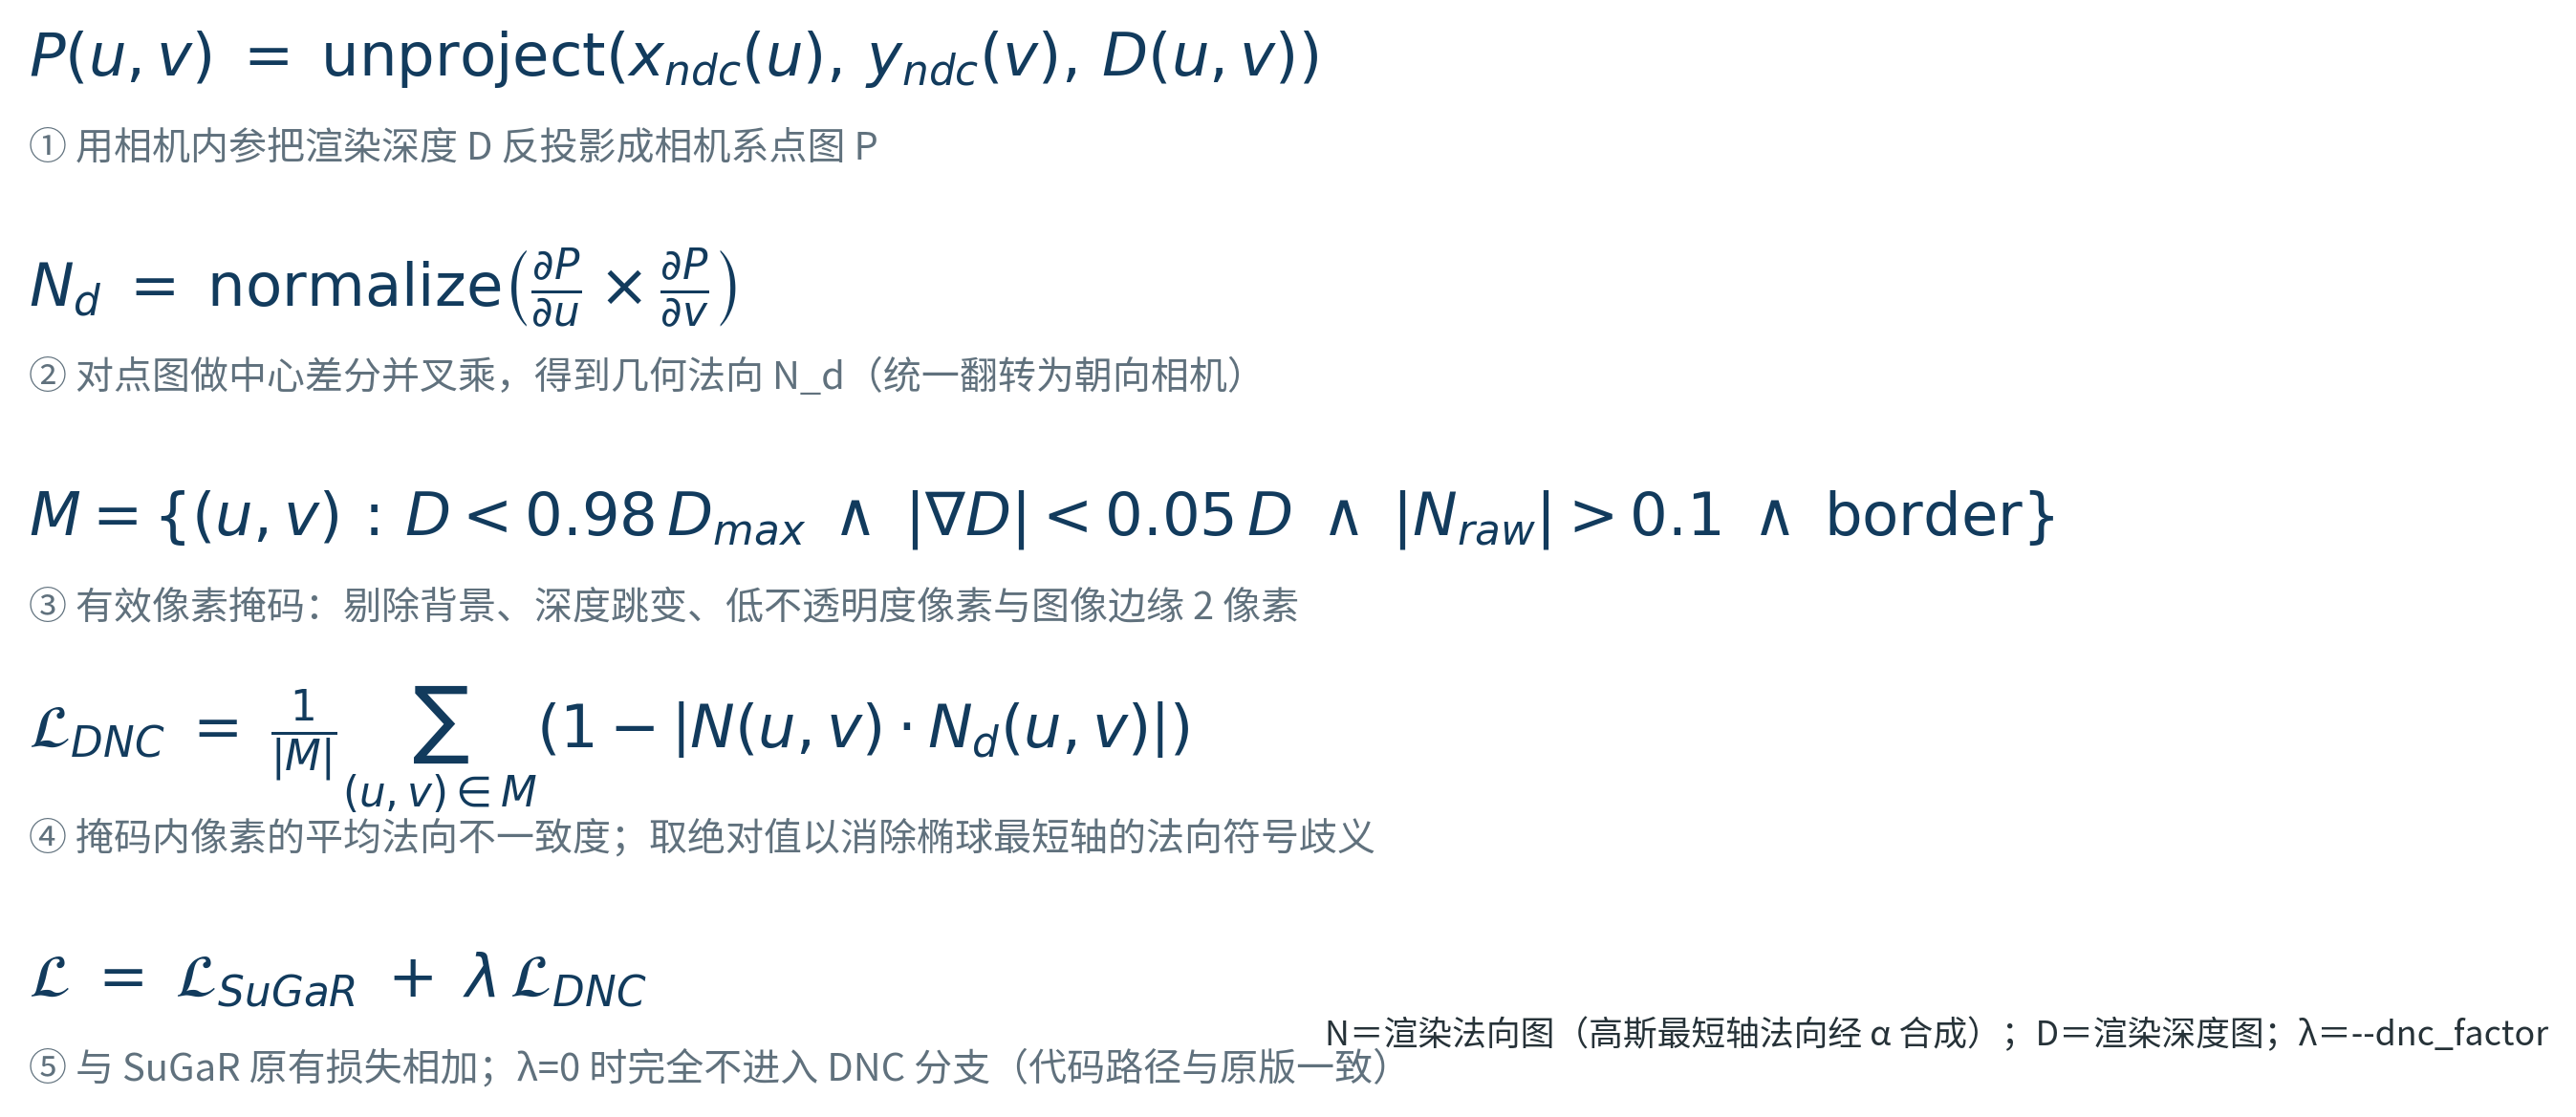
\includegraphics[width=0.85\linewidth]{figures/fig0_dnc_formula.png}
\caption{深度-法向一致性正则 L\_DNC 的定义与有效像素掩码}
\label{fig:1}
\end{figure}
实现要点：$\lambda$ = 0 时完全不进入 DNC 分支（不渲染额外的深度图与法向图），保证基线的代码路径与原版 SuGaR 完全一致；DNC 从第 9000 迭代起生效，与 SuGaR 自身的 SDF 正则同期；每 100 迭代把 L\_DNC、有效像素占比与两项 SDF 损失写入 dnc\_log.csv，每 1000 迭代把 D / N / N\_d / 掩码 四张图落盘。

\subsection{3.4 代码改动范围}
{
\begin{longtable}{>{\raggedright\arraybackslash}p{10.63cm}>{\raggedright\arraybackslash}p{1.99cm}>{\raggedright\arraybackslash}p{1.99cm}}
\caption{改动涉及的文件与行数统计}\label{tab:3}\\
\toprule
\textbf{文件} & \textbf{新增行} & \textbf{删除行} \\
\midrule
\endfirsthead
\multicolumn{3}{l}{\footnotesize（续表 3）}\\
\toprule
\textbf{文件} & \textbf{新增行} & \textbf{删除行} \\
\midrule
\endhead
\bottomrule
\endlastfoot
sugar\_trainers/coarse\_density.py & 225 & 1 \\
sugar\_utils/dnc\_utils.py & 394 & 0 \\
train\_coarse\_density.py & 31 & 0 \\
\end{longtable}
}
来源：notes/dnc\_stage3.patch（git diff 留痕）。合计新增 650 行、删除 1 行；改动只涉及训练入口参数、coarse 训练循环与一个新增的独立工具模块，未触碰网格提取与评测代码。

\section{4 实验设置与对照}
{\small
\begin{longtable}{>{\raggedright\arraybackslash}p{2.32cm}>{\raggedright\arraybackslash}p{2.75cm}>{\raggedright\arraybackslash}p{2.32cm}>{\raggedright\arraybackslash}p{1.74cm}>{\raggedright\arraybackslash}p{4.63cm}}
\caption{三组对照的配置差异（其余超参完全一致）}\label{tab:4}\\
\toprule
\textbf{组别} & \textbf{run 目录名} & \textbf{$\lambda$ (--dnc\_factor)} & \textbf{DNC 起始迭代} & \textbf{输出目录} \\
\midrule
\endfirsthead
\multicolumn{5}{l}{\footnotesize（续表 4）}\\
\toprule
\textbf{组别} & \textbf{run 目录名} & \textbf{$\lambda$ (--dnc\_factor)} & \textbf{DNC 起始迭代} & \textbf{输出目录} \\
\midrule
\endhead
\bottomrule
\endlastfoot
基线 $\lambda$=0 & coarse\_base\_seed0 & 0 & \textemdash{} & outputs/runs/coarse\_base\_seed0 \\
本工作 $\lambda$=0.05 & coarse\_dnc005 & 0.05 & 9000 & outputs/runs/coarse\_dnc005 \\
本工作 $\lambda$=0.2 & coarse\_dnc02 & 0.2 & 9000 & outputs/runs/coarse\_dnc02 \\
$\lambda$=0.2+detach & coarse\_dnc02\_detach & 0.2 & 9000 & outputs/runs/coarse\_dnc02\_detach \\
官方 DNC & coarse\_official\_dnc & 0.05 & 9000 & outputs/runs/coarse\_official\_dnc \\
3DGS 7k(参考) & vanilla3dgs7k & \textemdash{} & \textemdash{} & 未完成 \\
基线(阶段2 留档) & coarse\_baseline & \textemdash{} & \textemdash{} & outputs/runs/coarse\_baseline \\
\end{longtable}
}
共同固定量：同一 3DGS 7000 迭代检查点、seed=0、总迭代 15000、estimation\_factor=0.2、normal\_factor=0.2、网格提取 surface\_level=0.3 与 decimation 200000、同一 llffhold=8 划分。

留档说明：阶段 2 中在未打补丁的原版代码上跑过一次基线（run 名 coarse\_baseline），该结果仅作为“补丁未改变 $\lambda$=0 代码路径”的旁证留档，不参与三组正式对照；正式对照的三组统一使用打补丁后的代码与 seed=0。

阶段 2 用官方原版代码跑的 coarse\_baseline（无 seed、无插桩）与打补丁后 $\lambda$=0 的 coarse\_base\_seed0 相比：PSNR 24.653 vs 24.620，SSIM 0.8564 vs 0.8555，距离中位数 0.0684\% vs 0.0687\%，连通分量 2237 vs 2233，碎片 2147 vs 2137，高斯数 429,075 vs 429,423。差异均在 CUDA 光栅化非确定性与随机采样带来的抖动量级内，据此判断 $\lambda$=0 时补丁没有改变原有代码路径（日志中也无任何 DNC 分支输出）。

\subsection{4.1 过程记录：首轮 $\lambda$ 组被中断与重跑}
本次考核在计算集群的交互式作业中进行。首轮三组对照采用双卡并行调度（$\lambda$=0 独占一卡，两个 $\lambda$>0 组共享另一卡），但两个 $\lambda$>0 组的训练在接近收尾时随作业的 walltime 到期被强制终止，未能写出最终检查点。恢复作业后只分配到单张 GPU，因此改为顺序重跑两个 $\lambda$>0 组：先 $\lambda$=0.2，再 $\lambda$=0.05，其余超参、种子、数据划分与网格提取参数与首轮完全一致。$\lambda$=0 组在首轮已完整跑完训练与网格提取，未受影响，不需要重跑。

按照考核要求保留失败记录，首轮被中断的两个目录原样保留（仅重命名以避免与重跑结果混淆），其中的逐迭代日志与 DNC 中间量快照仍可作为“训练确实进行到了什么程度”的证据：

{\footnotesize
\begin{longtable}{>{\raggedright\arraybackslash}p{3.36cm}>{\raggedright\arraybackslash}p{2.15cm}>{\raggedright\arraybackslash}p{1.08cm}>{\raggedright\arraybackslash}p{1.61cm}>{\raggedright\arraybackslash}p{1.61cm}>{\raggedright\arraybackslash}p{3.50cm}}
\caption{首轮被中断的 $\lambda$ 组残留记录（保留为失败证据，不参与正式对照）}\label{tab:5}\\
\toprule
\textbf{残留目录} & \textbf{dnc\_log 最后迭代} & \textbf{日志行数} & \textbf{中间量快照数} & \textbf{最后快照迭代} & \textbf{是否有 15000.pt} \\
\midrule
\endfirsthead
\multicolumn{6}{l}{\footnotesize（续表 5）}\\
\toprule
\textbf{残留目录} & \textbf{dnc\_log 最后迭代} & \textbf{日志行数} & \textbf{中间量快照数} & \textbf{最后快照迭代} & \textbf{是否有 15000.pt} \\
\midrule
\endhead
\bottomrule
\endlastfoot
coarse\_dnc005\_killed\_0649 & 14900 & 59 & 5 & 14000 & 否（被中断，无最终检查点） \\
coarse\_dnc02\_killed\_0649 & 14900 & 59 & 5 & 14000 & 否（被中断，无最终检查点） \\
\end{longtable}
}
表中数字由脚本直接从磁盘上的残留文件统计得到（dnc\_log.csv 的最大迭代号、dnc\_vis/ 下 iter*\_depth.png 的数量与最大迭代号），不是人工记录。这些目录只用于说明中断发生的时点，其指标不进入任何结论。

06:49 首个 PBS 作业 walltime 到期被强杀，此时 $\lambda$=0.05 与 $\lambda$=0.2 两组均已训练到 14900/15000 迭代；由于 SuGaR 不保存中间检查点，两组全部重跑。07:57 起在新作业（hopper-13，仅 1 张 H200）上顺序重跑：$\lambda$=0.2 于 08:18 完成训练与提取，$\lambda$=0.05 于 08:33 完成训练；其网格提取因运行中的脚本被并发编辑而中断，08:34--08:40 手动补跑。诊断组 $\lambda$=0.2+detach 于 08:40--09:00 独占 GPU 完成。首轮被杀的两组残留目录与日志以 *\_killed\_0649 后缀保留，首轮 $\lambda$=0.2 在 14900 迭代时已呈现与重跑组一致的坍缩形态，说明该现象可复现，非偶然。由于重跑发生在不同节点、且 OMP 线程数在组间不一致（$\lambda$=0 组为 24，其余为 12），训练代价列只能作量级参考，不是受控对照。

写作后期追加的两组实验的时间线（逐字取自各阶段 SELF\_CHECK 的日志表）：① 官方 dn\_consistency 对照组 \textemdash{}\textemdash{} 等待脚本 08:34:34 进入 GPU 轮询，08:58:55 检测到 detach 组结束信号后开始训练，09:13:35 训练结束（880 秒），09:18:52 网格提取结束（317 秒），09:19:39 评测完成；② 提取端扫参（Frosting 自动 Poisson 深度）\textemdash{}\textemdash{} 09:16 完成移植与自检，四组提取与评测在 09:2x--10:0x 顺序完成，全部复用同一个 $\lambda$=0 的 coarse 模型，不重训。

\section{5 结果}
\subsection{5.1 定量结果}
{\footnotesize
\begin{longtable}{>{\raggedright\arraybackslash}p{2.36cm}>{\raggedright\arraybackslash}p{1.63cm}>{\raggedright\arraybackslash}p{2.00cm}>{\raggedright\arraybackslash}p{2.00cm}>{\raggedright\arraybackslash}p{1.09cm}>{\raggedright\arraybackslash}p{2.00cm}>{\raggedright\arraybackslash}p{1.82cm}}
\caption{测试视角上的渲染质量指标}\label{tab:6}\\
\toprule
\textbf{组别} & \textbf{高斯数} & \textbf{PSNR (dB) $\uparrow$} & \textbf{PSNR 标准差} & \textbf{SSIM $\uparrow$} & \textbf{LPIPS-VGG $\downarrow$} & \textbf{测试视角数} \\
\midrule
\endfirsthead
\multicolumn{7}{l}{\footnotesize（续表 6）}\\
\toprule
\textbf{组别} & \textbf{高斯数} & \textbf{PSNR (dB) $\uparrow$} & \textbf{PSNR 标准差} & \textbf{SSIM $\uparrow$} & \textbf{LPIPS-VGG $\downarrow$} & \textbf{测试视角数} \\
\midrule
\endhead
\bottomrule
\endlastfoot
基线 $\lambda$=0 & 429,423 & 24.620 & 1.106 & 0.8555 & 0.2032 & 32 \\
本工作 $\lambda$=0.05 & 429,395 & 22.447 & 0.976 & 0.7709 & 0.3458 & 32 \\
本工作 $\lambda$=0.2 & 429,416 & 13.244 & 1.123 & 0.4741 & 0.6465 & 32 \\
$\lambda$=0.2+detach & 429,406 & 24.399 & 1.101 & 0.8495 & 0.2133 & 32 \\
官方 DNC & 429,411 & 24.378 & 1.109 & 0.8485 & 0.2175 & 32 \\
3DGS 7k(参考) & 1,854,920 & 23.900 & 1.127 & 0.8499 & 0.2012 & 32 \\
\end{longtable}
}
$\uparrow$ 越高越好，$\downarrow$ 越低越好。PSNR 标准差为 32 个测试视角之间的样本标准差（ddof=0）。vanilla3dgs7k 行为 3DGS 训练 7000 迭代的原始高斯，仅作参考基准，不是 SuGaR 结果。

{\scriptsize
\begin{longtable}{>{\raggedright\arraybackslash}p{1.80cm}>{\raggedright\arraybackslash}p{0.97cm}>{\raggedright\arraybackslash}p{1.25cm}>{\raggedright\arraybackslash}p{0.97cm}>{\raggedright\arraybackslash}p{2.35cm}>{\raggedright\arraybackslash}p{1.94cm}>{\raggedright\arraybackslash}p{1.66cm}>{\raggedright\arraybackslash}p{1.52cm}}
\caption{几何精度：COLMAP 稀疏点到网格的距离与精度比例}\label{tab:7}\\
\toprule
\textbf{组别} & \textbf{G1 均值} & \textbf{G1 中位数} & \textbf{G1 P90} & \textbf{G1 中位数(相对 \%)} & \textbf{G2 <0.5\% (\%) $\uparrow$} & \textbf{G2 <1\% (\%) $\uparrow$} & \textbf{G3 前景均值} \\
\midrule
\endfirsthead
\multicolumn{8}{l}{\footnotesize（续表 7）}\\
\toprule
\textbf{组别} & \textbf{G1 均值} & \textbf{G1 中位数} & \textbf{G1 P90} & \textbf{G1 中位数(相对 \%)} & \textbf{G2 <0.5\% (\%) $\uparrow$} & \textbf{G2 <1\% (\%) $\uparrow$} & \textbf{G3 前景均值} \\
\midrule
\endhead
\bottomrule
\endlastfoot
基线 $\lambda$=0 & 0.01035 & 0.00402 & 0.01938 & 0.0687 & 94.13 & 97.74 & 0.10666 \\
本工作 $\lambda$=0.05 & 0.02400 & 0.00831 & 0.07004 & 0.1421 & 75.81 & 87.28 & 0.11652 \\
本工作 $\lambda$=0.2 & 0.10732 & 0.04908 & 0.24174 & 0.8392 & 33.80 & 55.47 & 0.39168 \\
$\lambda$=0.2+detach & 0.01175 & 0.00491 & 0.02188 & 0.0839 & 93.26 & 97.54 & 0.12121 \\
官方 DNC & 0.01088 & 0.00400 & 0.02142 & 0.0684 & 93.35 & 97.49 & 0.10299 \\
\end{longtable}
}
G1 为点到网格表面的无符号距离（场景单位，$\downarrow$ 越小越好），相对值以相机空间尺度归一化；G2 为距离小于相机空间尺度 0.5\% / 1\% 的点占比（$\uparrow$）；G3 为网格顶点到最近稀疏点的平均距离（仅统计落在前景包围盒内的顶点，$\downarrow$）。稀疏点本身稀疏、非稠密真值，G3 只作参考，不能单独判优劣。

{\scriptsize
\begin{longtable}{>{\raggedright\arraybackslash}p{1.45cm}>{\raggedright\arraybackslash}p{0.84cm}>{\raggedright\arraybackslash}p{0.84cm}>{\raggedright\arraybackslash}p{1.34cm}>{\raggedright\arraybackslash}p{2.45cm}>{\raggedright\arraybackslash}p{1.78cm}>{\raggedright\arraybackslash}p{1.34cm}>{\raggedright\arraybackslash}p{1.11cm}>{\raggedright\arraybackslash}p{0.89cm}}
\caption{网格拓扑统计（漂浮碎片是 H1 的主要观测量）}\label{tab:8}\\
\toprule
\textbf{组别} & \textbf{顶点数} & \textbf{面数} & \textbf{连通分量数 $\downarrow$} & \textbf{最大分量面数占比 (\%) $\uparrow$} & \textbf{碎片 (<100 面) $\downarrow$} & \textbf{碎片总面数 $\downarrow$} & \textbf{非流形边 $\downarrow$} & \textbf{边界边 $\downarrow$} \\
\midrule
\endfirsthead
\multicolumn{9}{l}{\footnotesize（续表 8）}\\
\toprule
\textbf{组别} & \textbf{顶点数} & \textbf{面数} & \textbf{连通分量数 $\downarrow$} & \textbf{最大分量面数占比 (\%) $\uparrow$} & \textbf{碎片 (<100 面) $\downarrow$} & \textbf{碎片总面数 $\downarrow$} & \textbf{非流形边 $\downarrow$} & \textbf{边界边 $\downarrow$} \\
\midrule
\endhead
\bottomrule
\endlastfoot
基线 $\lambda$=0 & 205,548 & 370,128 & 2,233 & 41.69 & 2,137 & 29,408 & 0 & 38,596 \\
本工作 $\lambda$=0.05 & 211,274 & 381,723 & 2,403 & 45.25 & 2,324 & 23,944 & 0 & 35,449 \\
本工作 $\lambda$=0.2 & 120,059 & 222,535 & 1,192 & 84.58 & 1,177 & 8,343 & 0 & 23,485 \\
$\lambda$=0.2+detach & 208,382 & 375,966 & 2,242 & 41.77 & 2,142 & 26,262 & 0 & 40,452 \\
官方 DNC & 205,113 & 370,554 & 1,872 & 44.59 & 1,787 & 24,117 & 0 & 35,934 \\
\end{longtable}
}
{\footnotesize
\begin{longtable}{>{\raggedright\arraybackslash}p{1.58cm}>{\raggedright\arraybackslash}p{1.70cm}>{\raggedright\arraybackslash}p{1.95cm}>{\raggedright\arraybackslash}p{1.70cm}>{\raggedright\arraybackslash}p{2.07cm}>{\raggedright\arraybackslash}p{1.95cm}>{\raggedright\arraybackslash}p{1.95cm}}
\caption{网格法向平滑度（相邻面二面角统计）}\label{tab:9}\\
\toprule
\textbf{组别} & \textbf{二面角均值 ($^\circ$)} & \textbf{二面角中位数 ($^\circ$)} & \textbf{二面角 P90 ($^\circ$)} & \textbf{|二面角| 均值 ($^\circ$)} & \textbf{|二面角| P90 ($^\circ$)} & \textbf{raw>90$^\circ$ 占比 (\%)} \\
\midrule
\endfirsthead
\multicolumn{7}{l}{\footnotesize（续表 9）}\\
\toprule
\textbf{组别} & \textbf{二面角均值 ($^\circ$)} & \textbf{二面角中位数 ($^\circ$)} & \textbf{二面角 P90 ($^\circ$)} & \textbf{|二面角| 均值 ($^\circ$)} & \textbf{|二面角| P90 ($^\circ$)} & \textbf{raw>90$^\circ$ 占比 (\%)} \\
\midrule
\endhead
\bottomrule
\endlastfoot
基线 $\lambda$=0 & 45.98 & 31.31 & 112.84 & 33.60 & 75.18 & 16.21 \\
本工作 $\lambda$=0.05 & 49.52 & 36.39 & 116.84 & 36.34 & 77.11 & 18.35 \\
本工作 $\lambda$=0.2 & 52.58 & 36.44 & 131.55 & 34.41 & 76.58 & 22.70 \\
$\lambda$=0.2+detach & 47.67 & 33.24 & 116.12 & 34.50 & 75.92 & 17.38 \\
官方 DNC & 40.41 & 24.94 & 103.01 & 30.22 & 72.28 & 13.15 \\
\end{longtable}
}
raw 为相邻面法向夹角（依赖三角形绕序），|二面角| 取 min(raw, 180$-$raw)（与绕序无关）。数值越低表示表面越平滑，但过低可能意味着细节被过度平滑，需结合图 3 与图 6 判断。

{\footnotesize
\begin{longtable}{>{\raggedright\arraybackslash}p{2.37cm}>{\raggedright\arraybackslash}p{1.09cm}>{\raggedright\arraybackslash}p{2.55cm}>{\raggedright\arraybackslash}p{2.74cm}>{\raggedright\arraybackslash}p{2.37cm}>{\raggedright\arraybackslash}p{2.19cm}}
\caption{训练代价（coarse SuGaR 阶段，7000$\rightarrow$15000 共 8000 迭代）}\label{tab:10}\\
\toprule
\textbf{组别} & \textbf{$\lambda$} & \textbf{训练墙钟 (min)} & \textbf{每迭代耗时 (ms)} & \textbf{峰值显存 (GB)} & \textbf{结束时高斯数} \\
\midrule
\endfirsthead
\multicolumn{6}{l}{\footnotesize（续表 10）}\\
\toprule
\textbf{组别} & \textbf{$\lambda$} & \textbf{训练墙钟 (min)} & \textbf{每迭代耗时 (ms)} & \textbf{峰值显存 (GB)} & \textbf{结束时高斯数} \\
\midrule
\endhead
\bottomrule
\endlastfoot
基线 $\lambda$=0 & 0 & 12.15 & 91.1 & 7.42 & 429,423 \\
本工作 $\lambda$=0.05 & 0.05 & 13.93 & 104.5 & 7.62 & 429,395 \\
本工作 $\lambda$=0.2 & 0.2 & 14.38 & 107.9 & 8.38 & 429,416 \\
$\lambda$=0.2+detach & 0.2 & 12.89 & 96.7 & 7.58 & 429,406 \\
官方 DNC & 0.05 & 14.55 & 109.1 & 7.65 & 429,411 \\
3DGS 7k(参考) & 未完成 & 未完成 & 未完成 & 未完成 & 未完成 \\
\end{longtable}
}
调度方式在过程中发生过变化（见 4.1 节）：首轮两个 $\lambda$>0 组共享同一张 GPU 并行执行，重跑时改为单卡顺序执行。因此墙钟时间不可直接横向比较，每迭代耗时与峰值显存受调度影响较小，是更可比的代价指标。

渲染指标随 $\lambda$ 单调恶化：PSNR 24.62 $\rightarrow$ 22.45 $\rightarrow$ 13.24 dB，LPIPS 0.203 $\rightarrow$ 0.346 $\rightarrow$ 0.646。几何指标同向：稀疏点到网格距离中位数 0.0687\% $\rightarrow$ 0.1421\% $\rightarrow$ 0.8392\%，距离 <1\% 相机尺度的稀疏点比例 97.7\% $\rightarrow$ 87.3\% $\rightarrow$ 55.5\%。训练日志显示 $\lambda$=0.2 组高斯最大尺度从 8.35 增至 83.68、不透明度均值从 0.65 降至 0.45，即高斯被拉大且变透明。L\_dnc 末值 $\lambda$=0.2 组最低（0.046），$\lambda$=0.05 组 0.240，detach 组 0.292：\textbf{L\_dnc 越低，结果越差}，说明该损失在本设置下主要被"抹平深度"这条捷径最小化，而非被"法向对齐"最小化。detach 组切断深度梯度后，PSNR 回升 11.16 dB、每迭代耗时降低 10\%、显存少 811 MiB，但几何指标与 $\lambda$=0 持平或略差。

\subsection{5.2 定性结果}
\begin{figure}[H]
\centering
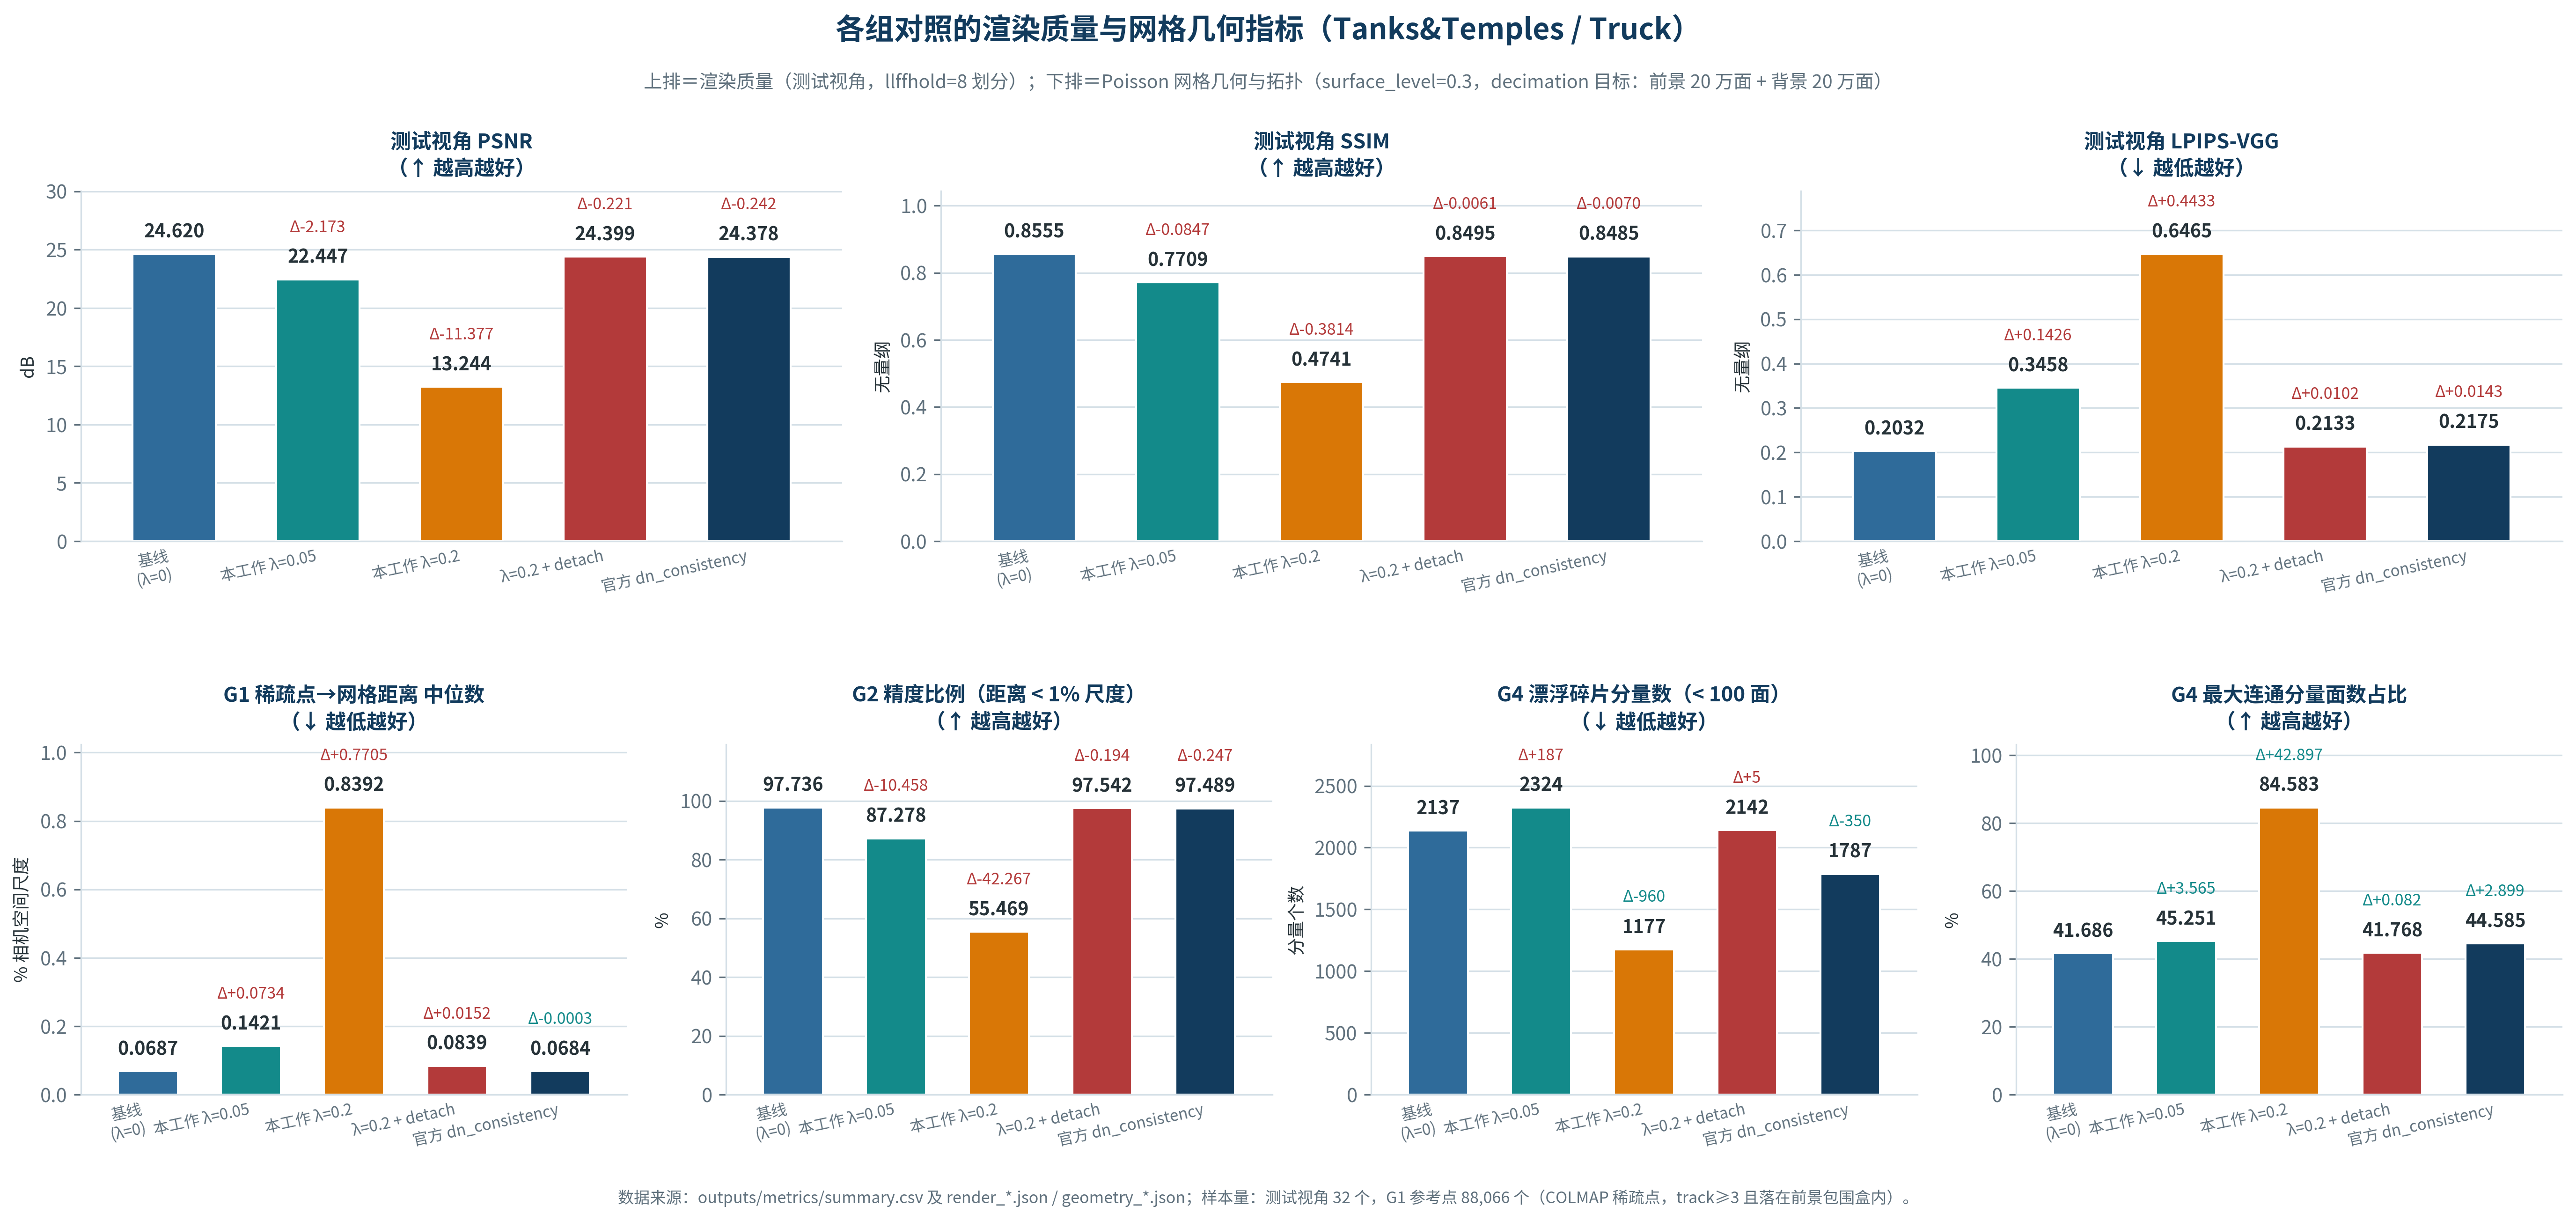
\includegraphics[width=1.0\linewidth]{figures/fig1_metrics.png}
\caption{各组对照的渲染质量与网格几何指标汇总（上排渲染、下排几何）（来源：scripts/deliverables/make\_figures.py）}
\label{fig:2}
\end{figure}
\begin{figure}[H]
\centering
\includegraphics[width=1.0\linewidth]{figures/fig2_render_compare.png}
\caption{固定测试视角的渲染结果与误差热图对比（误差图共用同一色条）}
\label{fig:3}
\end{figure}
\begin{figure}[H]
\centering
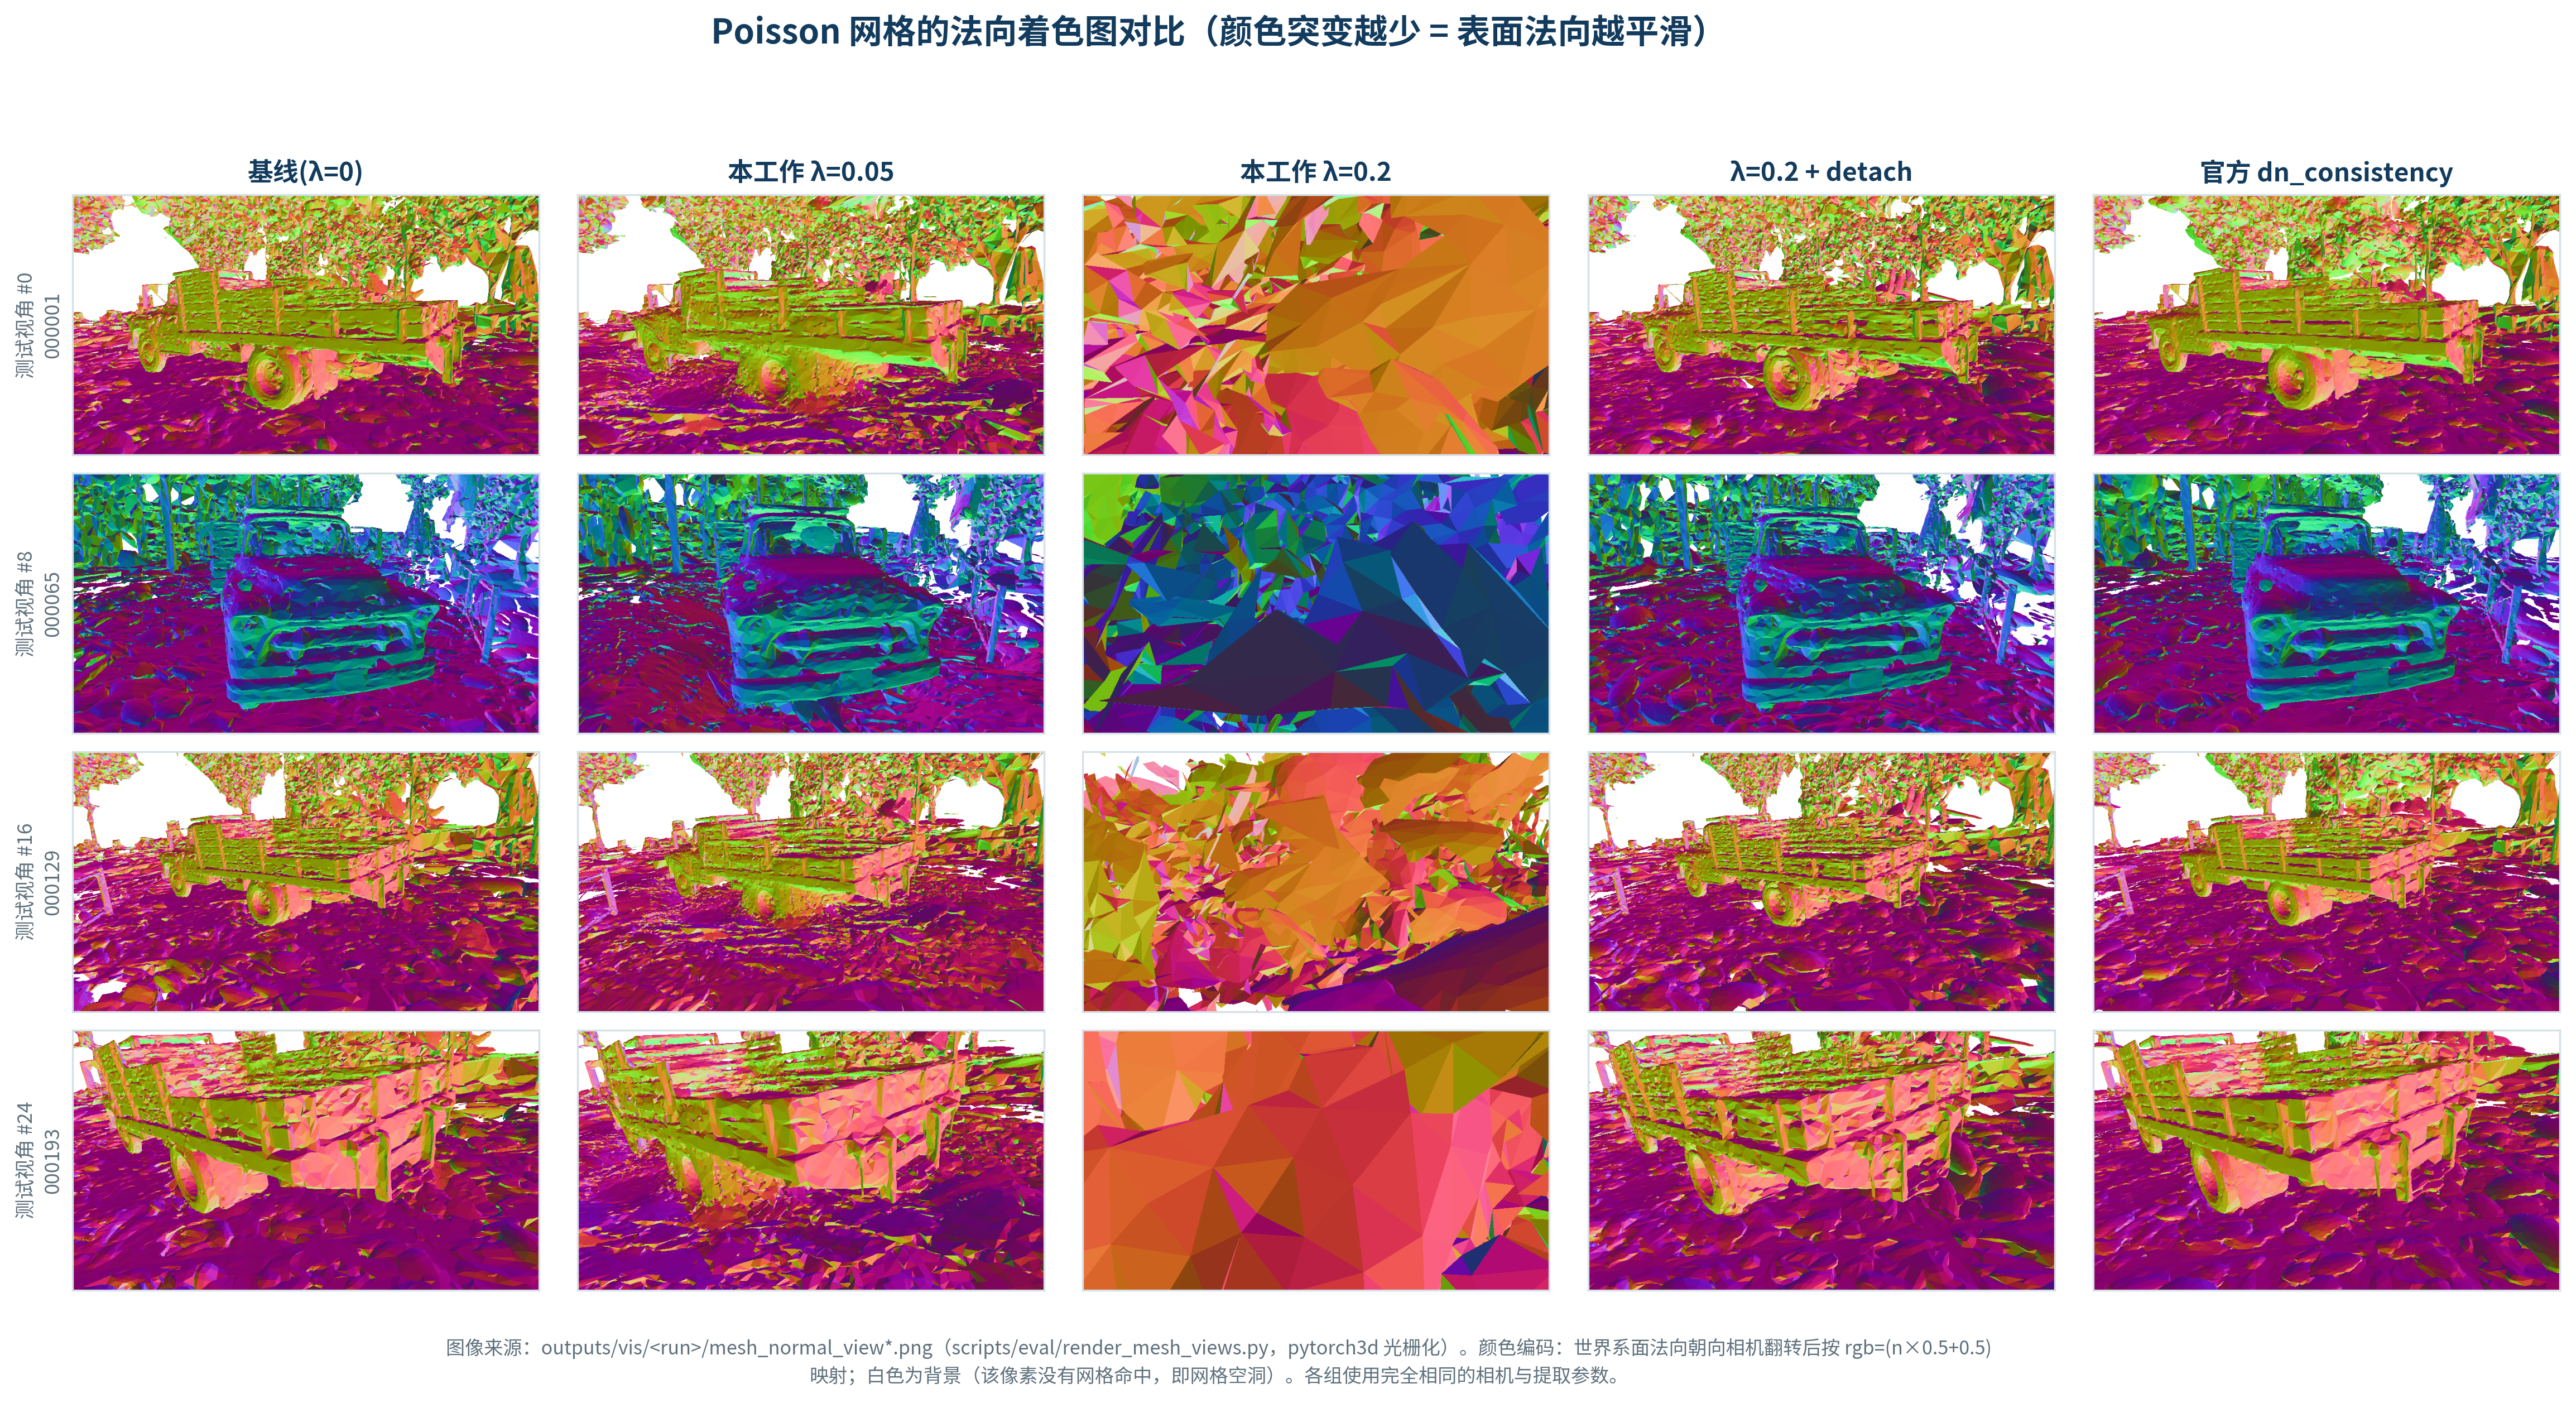
\includegraphics[width=1.0\linewidth]{figures/fig3_mesh_normal.png}
\caption{各组网格的法向着色图对比（白色区域为网格空洞）}
\label{fig:4}
\end{figure}
\begin{figure}[H]
\centering
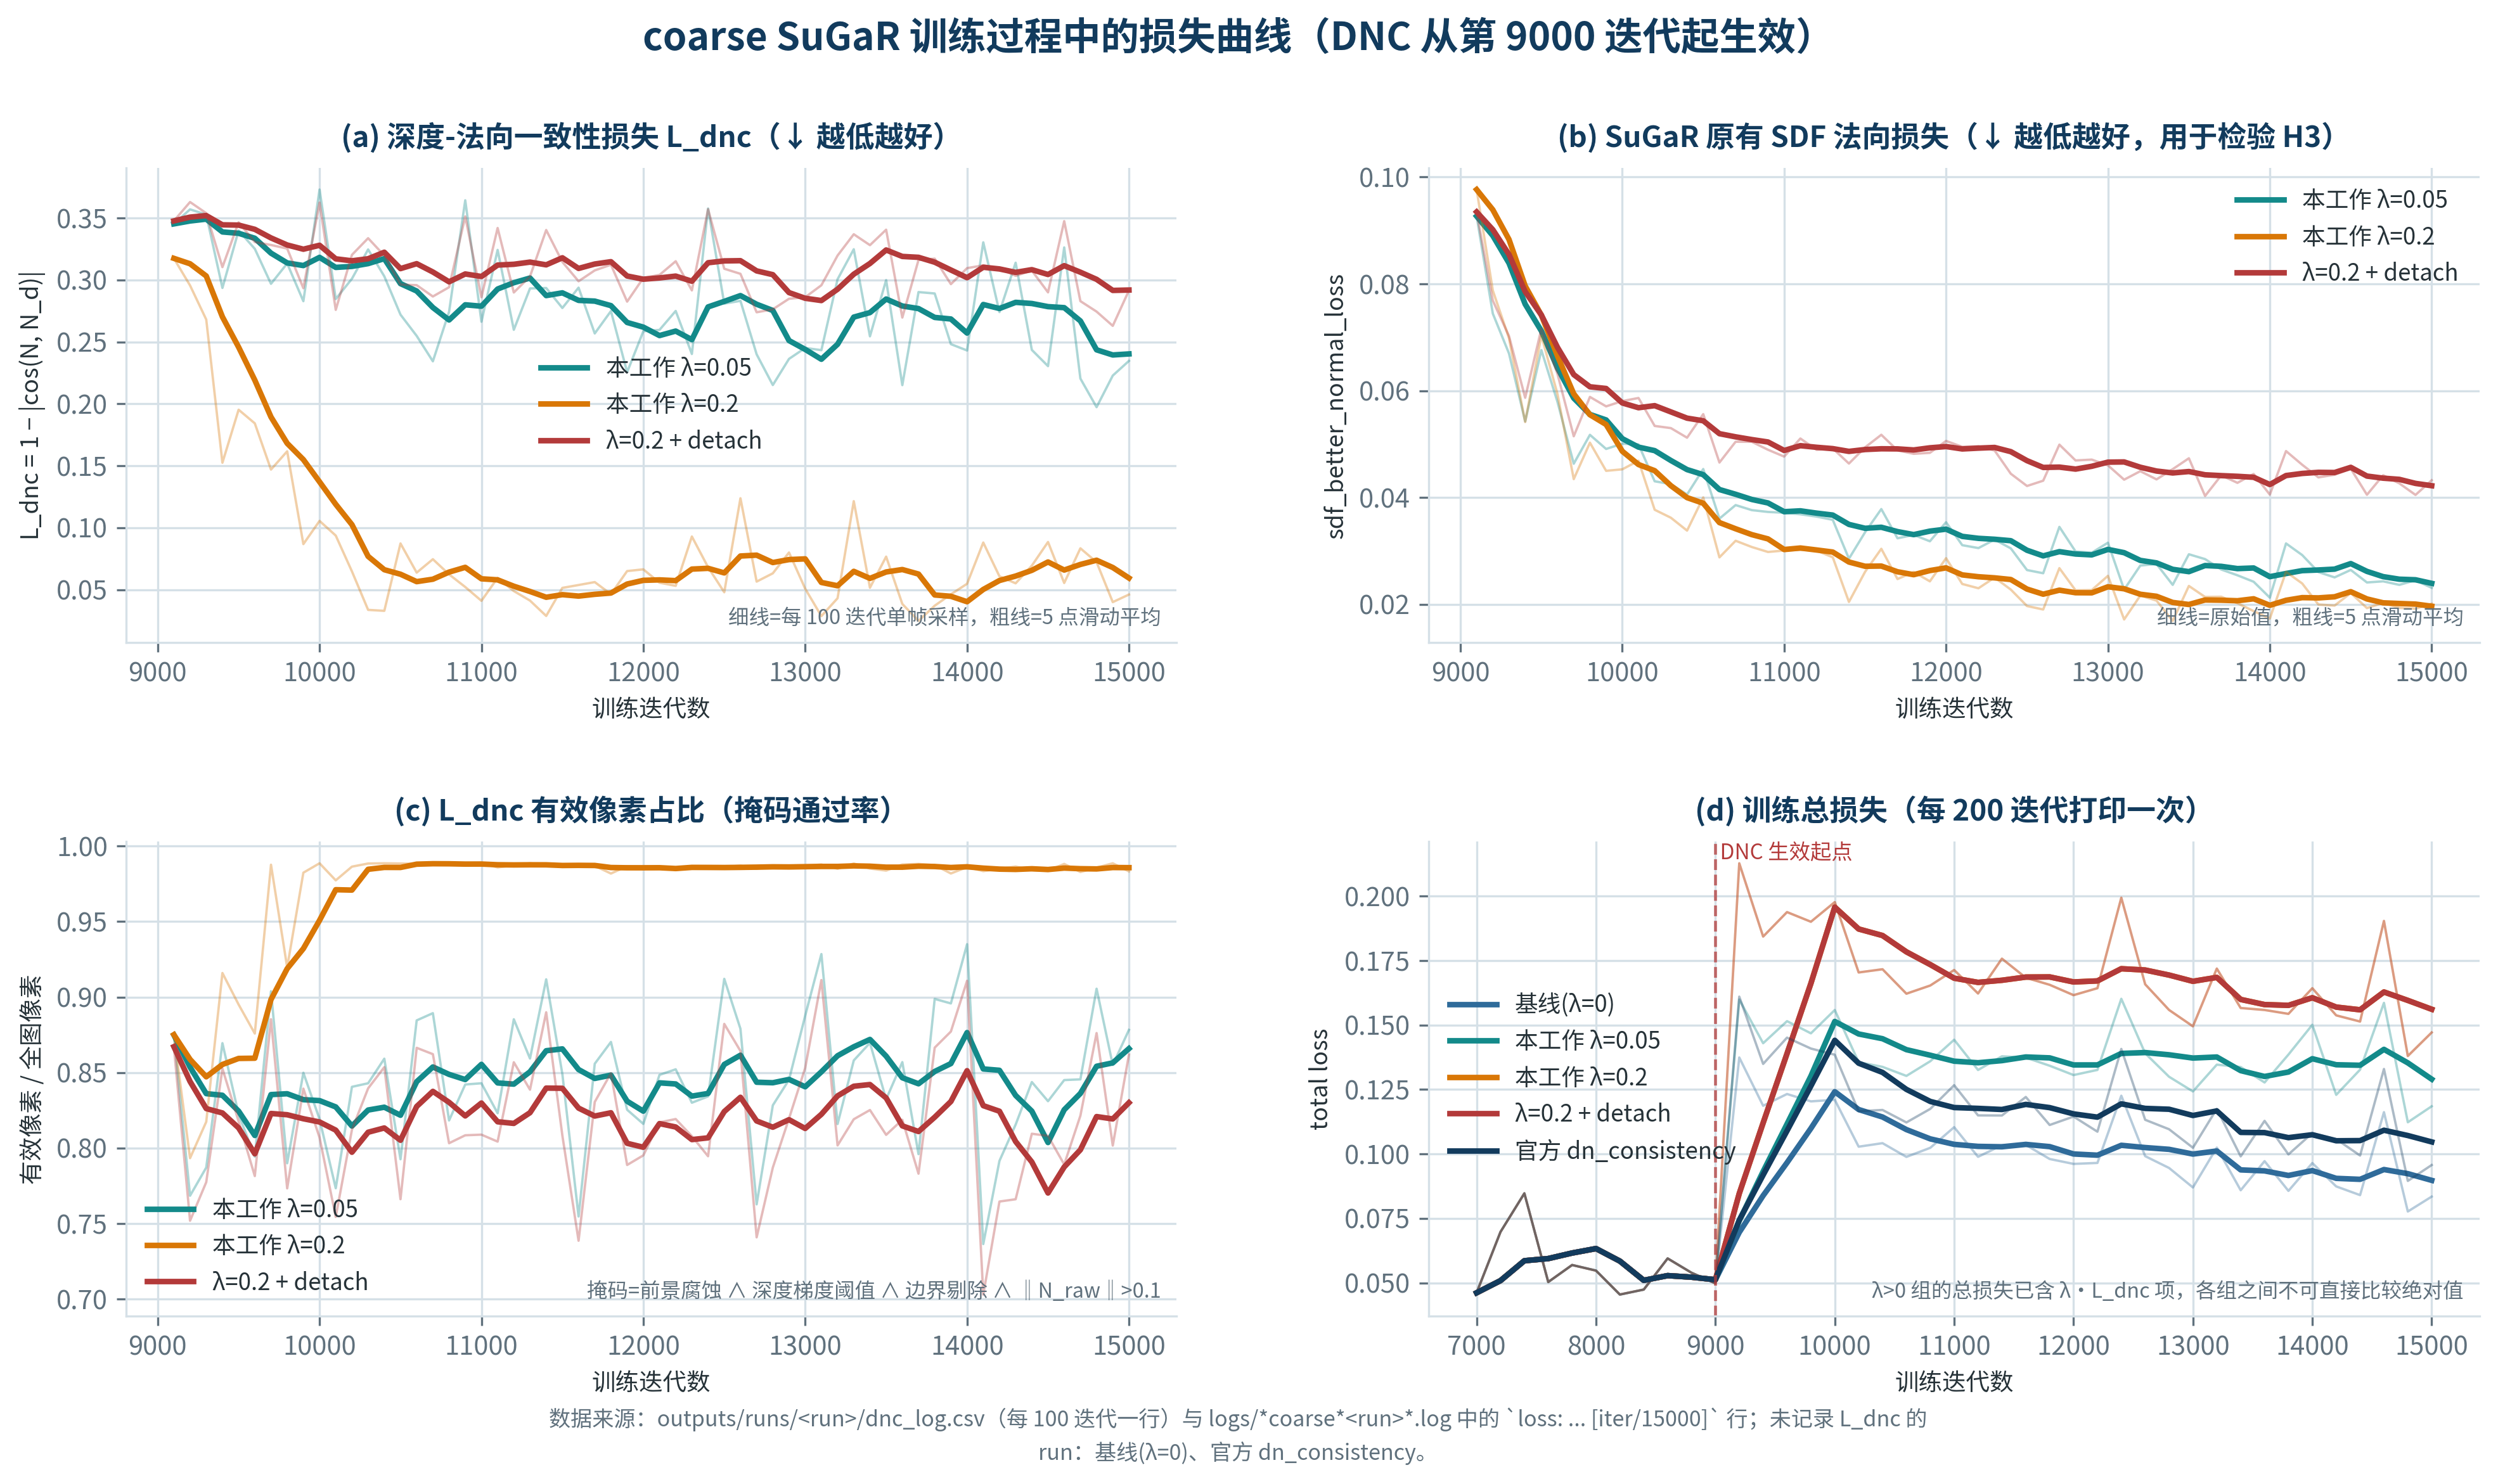
\includegraphics[width=1.0\linewidth]{figures/fig4_train_curves.png}
\caption{训练过程中的 L\_DNC、SDF 法向损失、有效像素占比与总损失曲线}
\label{fig:5}
\end{figure}
\begin{figure}[H]
\centering
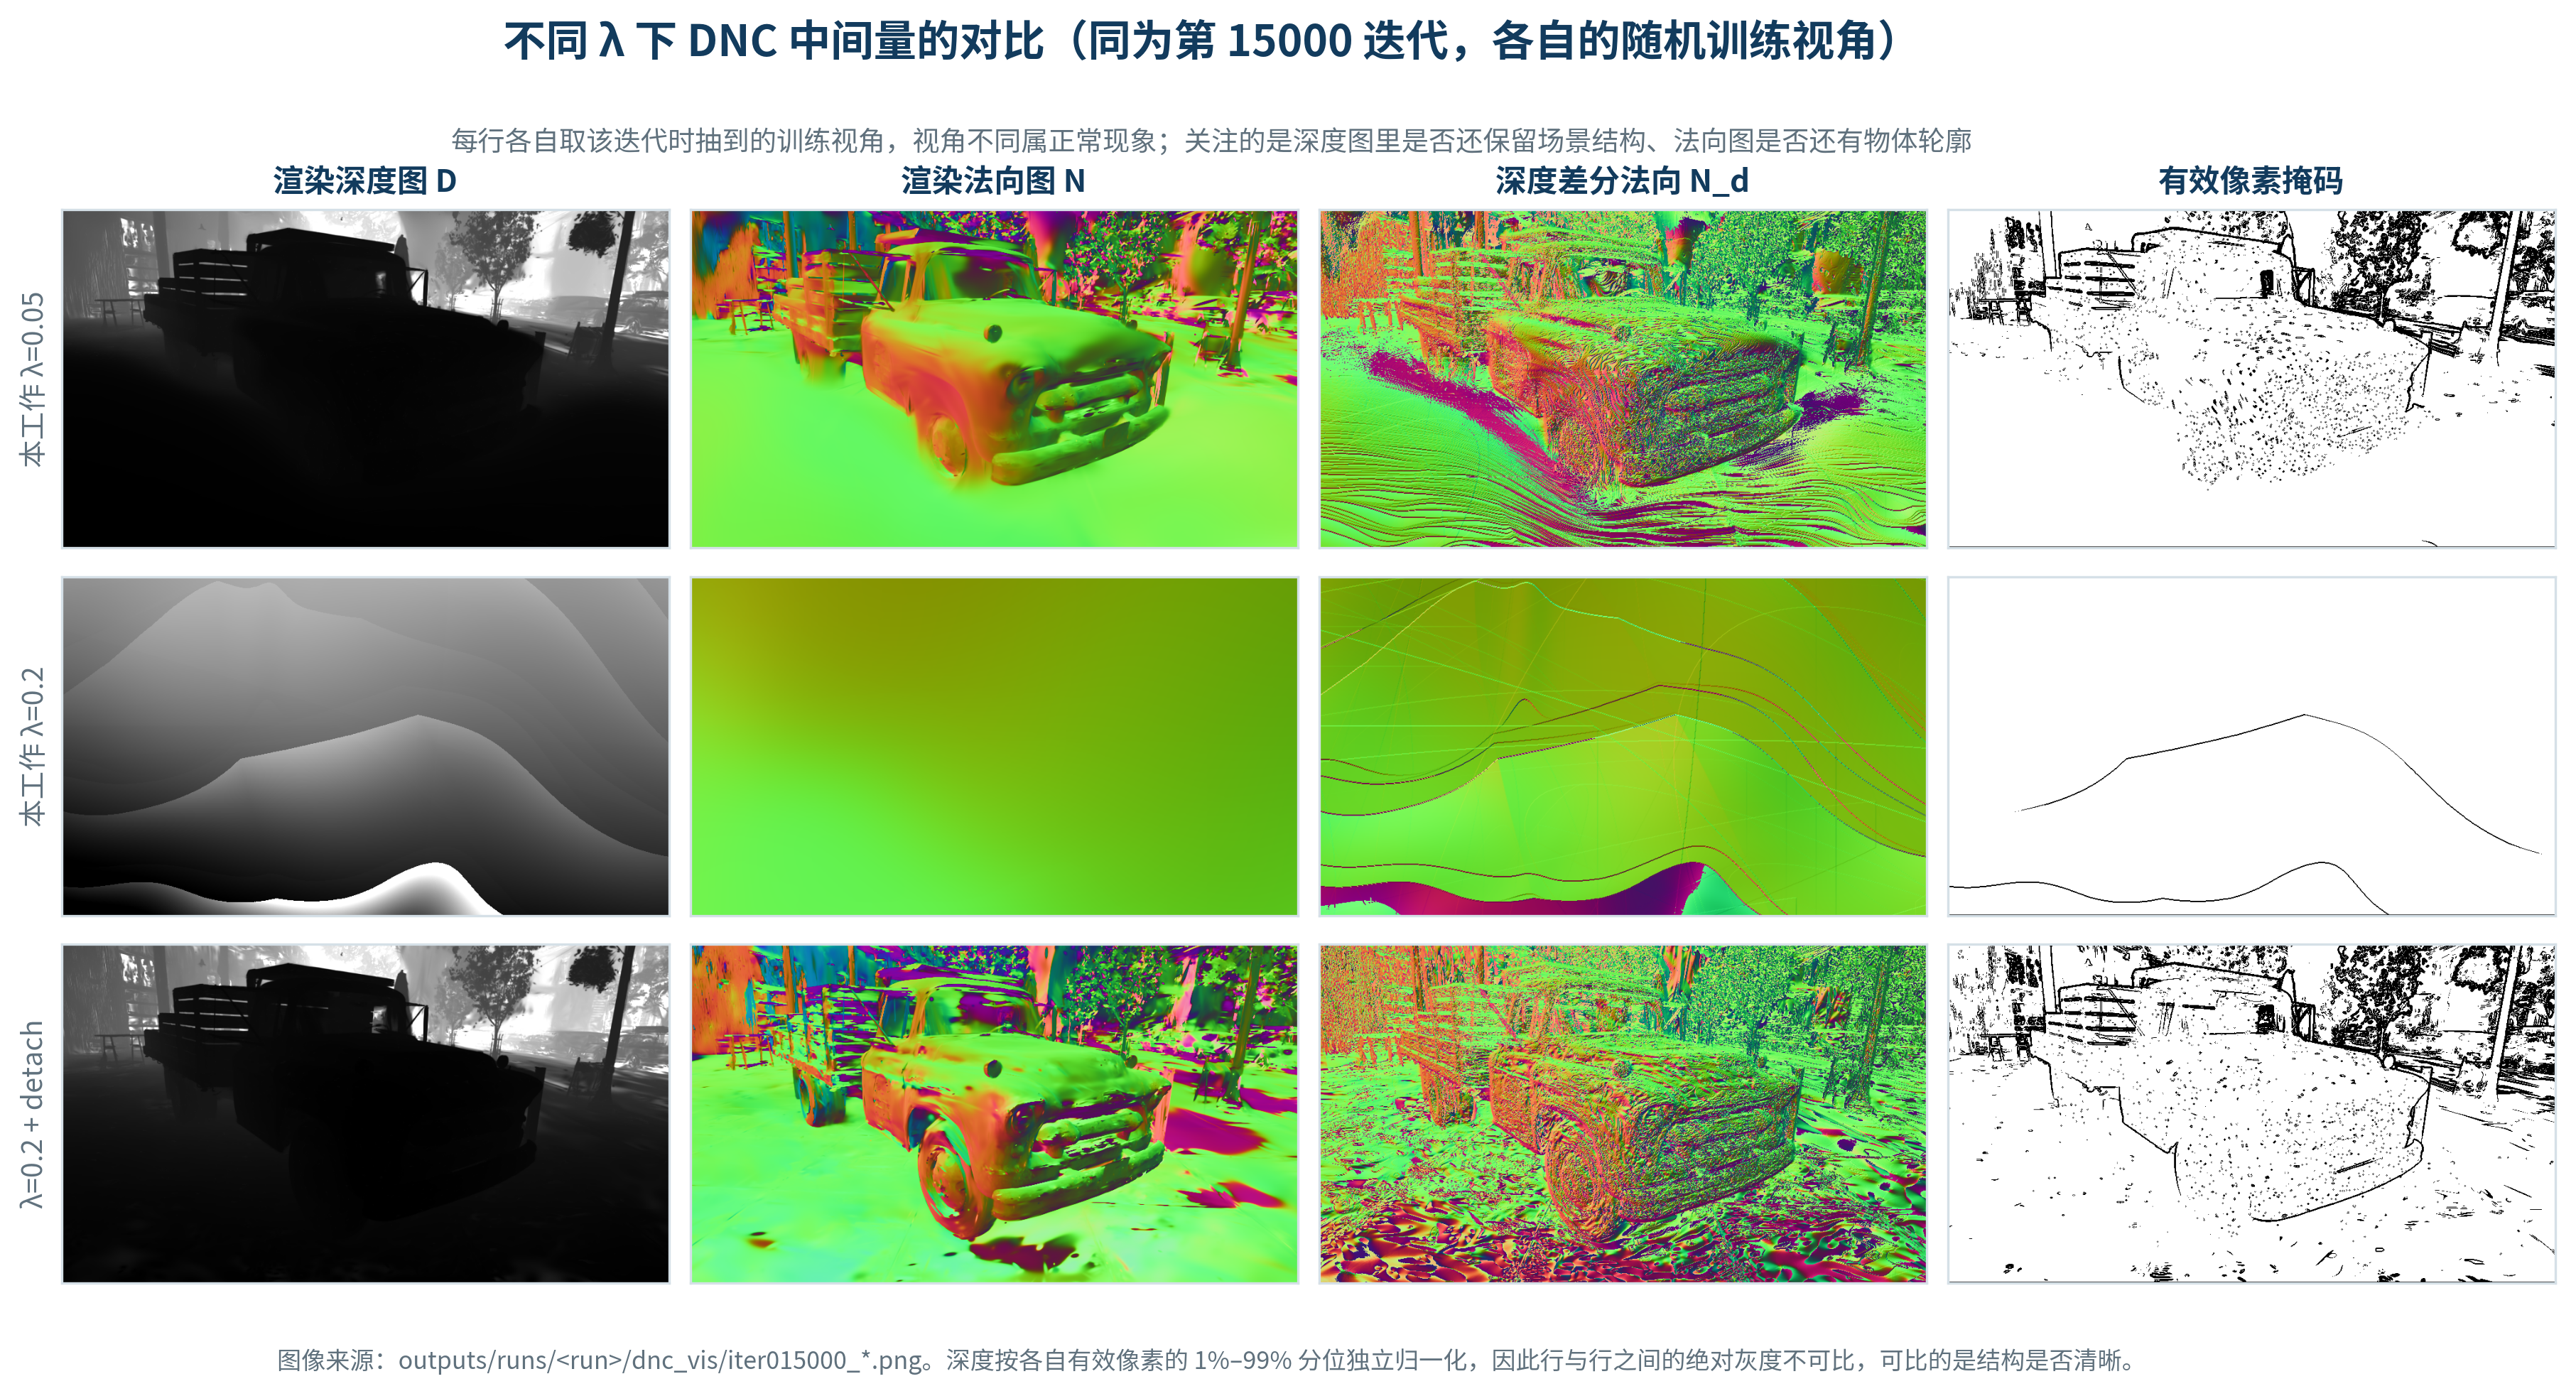
\includegraphics[width=1.0\linewidth]{figures/fig5_dnc_internals.png}
\caption{DNC 中间量逐组对比：深度 D、渲染法向 N、深度差分法向 N\_d 与有效掩码（第 15000 迭代）}
\label{fig:6}
\end{figure}
$\lambda$=0.05 的测试视角渲染中卡车本体基本正常，但地面被抹成一块均匀灰板，是退化的早期形态；$\lambda$=0.2 整幅画面糊成色块。DNC 中间量可视化显示：SuGaR 的深度图由每个高斯中心的视空间 z 经 alpha 合成得到，是分片常数的阶梯面，对其做有限差分得到的几何法向 N\_d 在平坦地面上呈密集条纹噪声。要降低 1$-$|cos(N, N\_d)|，把法向对准这种噪声代价很高，而让若干大尺度高斯把深度真正抹平则代价很低，优化因此走向后者。detach 组的深度图在 15000 迭代仍保留车头格栅、车轮、栏板、树干等结构（深度梯度 >0.02 的像素占 12.8\%，$\lambda$=0.2 非 detach 组仅 1.5\%），证实平凡解只在梯度流经深度时出现。

\subsection{5.3 官方 dn\_consistency 对照}
在写作后期核实到：SuGaR 官方仓库已经内置了同类正则 sugar\_trainers/coarse\_density\_and\_dn\_consistency.py（2024-09 加入仓库）。本工作的 DNC 属于独立实现，报告如实披露这一点，并把官方实现按完全相同的 3DGS 检查点、seed、迭代数与网格提取参数补跑成第五组对照，用来回答一个关键问题：失效到底是“思路不成立”还是“我的实现细节不对”。

{\small
\begin{longtable}{>{\raggedright\arraybackslash}p{1.48cm}>{\raggedright\arraybackslash}p{4.23cm}>{\raggedright\arraybackslash}p{4.23cm}>{\raggedright\arraybackslash}p{4.23cm}}
\caption{本工作 DNC 与官方 dn\_consistency 的实现差异清单}\label{tab:11}\\
\toprule
\textbf{差异项} & \textbf{本工作实现} & \textbf{官方 dn\_consistency 实现} & \textbf{可能的影响} \\
\midrule
\endfirsthead
\multicolumn{4}{l}{\footnotesize（续表 11）}\\
\toprule
\textbf{差异项} & \textbf{本工作实现} & \textbf{官方 dn\_consistency 实现} & \textbf{可能的影响} \\
\midrule
\endhead
\bottomrule
\endlastfoot
损失形式 & 1 $-$ |cos(N, N\_d)|，取绝对值以消除三维椭球最短轴的符号歧义 & 1 $-$ cos(N, N\_d)，不取绝对值 & 绝对值让“法向整体翻转”也成为零损失解，放宽了约束 \\
法向的合成方式 & 把三通道世界系法向光栅化后，再逐像素归一化 & 只光栅化法向的 x、y 两个分量（与深度 z 打包成一次三通道光栅化），再按单位长度解析恢复 z & 官方得到的逐像素法向天然是单位向量；本工作 $\alpha$ 合成后再归一化，低不透明度像素的方向不可靠 \\
有效像素掩码 & 有：背景、深度跳变、图像边缘 2 像素、$\|$N\_raw$\|$>0.1 四条 & 无：全图像素参与 & 掩码会随训练进程改变参与像素集合，可能与优化目标相互作用 \\
光栅化次数 & 额外两次（深度一次、法向一次） & 额外一次（深度与法向打包） & 本工作每迭代耗时高约 16\%，官方约 6\% \\
\end{longtable}
}
两版实现的权重、起始迭代（$\lambda$=0.05、第 9000 迭代起）与训练预算完全一致；哪一处差异是失效主因需要逐项消融，本次未完成，不下结论。

官方 sugar\_trainers/coarse\_density\_and\_dn\_consistency.py（2024-09 加入仓库，$\lambda$=0.05，9000 起，无掩码、不取绝对值、梯度同时流经深度与法向，深度 z 与法向 x、y 打包成一次三通道光栅化）在相同 3DGS 检查点、seed 与提取参数下：PSNR 24.378（$\lambda$=0 为 24.620）、SSIM 0.8485、LPIPS 0.2175；G1 距离中位数 0.0684\%（持平）、连通分量 2233$\rightarrow$1872（$-$16.2\%）、碎片 2137$\rightarrow$1787（$-$16.4\%）、二面角均值 33.60$^\circ$$\rightarrow$30.23$^\circ$（$-$10.1\%）；每迭代耗时较 $\lambda$=0 高约 6\%（本工作 $\lambda$=0.05 版高 16\%，因为多做一次光栅化）。这是全部对照组中唯一"几何变好、渲染几乎不掉"的一组。写作者在实验后期才核实到该实现的存在；本工作的 DNC 为独立实现，报告如实披露这一点。两版实现的差异清单见 P10；对这三处差异的逐项消融是最直接的下一步。

\subsection{5.4 提取端改动：Frosting 的自动 Poisson 深度}
除了训练端的 DNC，本工作还移植了一项提取端改动：把 SuGaR 里写死的泊松重建深度 （Poisson depth，默认 10）改成按场景尺度自动推算。来源注明：算法取自同一作者的后续工作 Frosting 仓库 （Anttwo/Frosting，frosting\_extractors/coarse\_shell.py 第 17--49 行），本工作按该段逻辑自行实现并接到 SuGaR 的 extract\_mesh.py 上，未复制代码。

\begin{itemize}
\setlength{\itemsep}{2pt}
  \item 自动深度的做法：取前景且不透明的高斯，按相机空间尺度归一化后求其最近邻距离的分位数，据此推出能分辨该尺度细节所需的八叉树深度，再对整数下取整并设下限；
  \item 本场景实测：参与统计的高斯 77,679 个，相机空间尺度 5.893，包围盒边长 12.956，推算出的原始深度 10.883，下取整后为 10 \textemdash{}\textemdash{} 与 SuGaR 的默认值一致，说明默认值在本场景恰好是合适的，自动化的价值在于换场景时不必手调；
  \item 顺带扫了顶点密度分位 quantile（默认 0.1，即丢掉密度最低的 10\% 顶点）取 0 的情形，用来观察“少裁剪”对碎片与精度的影响。
\end{itemize}
{\scriptsize
\begin{longtable}{>{\raggedright\arraybackslash}p{1.28cm}>{\raggedright\arraybackslash}p{0.86cm}>{\raggedright\arraybackslash}p{0.84cm}>{\raggedright\arraybackslash}p{1.04cm}>{\raggedright\arraybackslash}p{1.04cm}>{\raggedright\arraybackslash}p{0.98cm}>{\raggedright\arraybackslash}p{0.98cm}>{\raggedright\arraybackslash}p{0.92cm}>{\raggedright\arraybackslash}p{0.92cm}>{\raggedright\arraybackslash}p{1.04cm}>{\raggedright\arraybackslash}p{1.28cm}}
\caption{提取端扫参：同一个 $\lambda$=0 的 coarse 模型，只改网格提取参数}\label{tab:12}\\
\toprule
\textbf{提取参数组合} & \textbf{Poisson 深度 D} & \textbf{quantile} & \textbf{顶点数} & \textbf{面数} & \textbf{G1 中位数(\%) $\downarrow$} & \textbf{G2 <1\%(\%) $\uparrow$} & \textbf{连通分量 $\downarrow$} & \textbf{碎片 $\downarrow$} & \textbf{最大分量占比(\%) $\uparrow$} & \textbf{G5 |二面角| 均值($^\circ$) $\downarrow$} \\
\midrule
\endfirsthead
\multicolumn{11}{l}{\footnotesize（续表 12）}\\
\toprule
\textbf{提取参数组合} & \textbf{Poisson 深度 D} & \textbf{quantile} & \textbf{顶点数} & \textbf{面数} & \textbf{G1 中位数(\%) $\downarrow$} & \textbf{G2 <1\%(\%) $\uparrow$} & \textbf{连通分量 $\downarrow$} & \textbf{碎片 $\downarrow$} & \textbf{最大分量占比(\%) $\uparrow$} & \textbf{G5 |二面角| 均值($^\circ$) $\downarrow$} \\
\midrule
\endhead
\bottomrule
\endlastfoot
原版参数（对照基准） & 10（默认） & 0.1（默认） & 205,548 & 370,128 & 0.0687 & 97.736 & 2,233 & 2,137 & 41.69 & 33.60 \\
自动 Poisson 深度 & auto$\rightarrow$10 & 0.1 & 205,400（-0.1\%） & 369,922（-0.1\%） & 0.0689（+0.2\%） & 97.737（+0.00\%） & 2,267（+1.5\%） & 2,172（+1.6\%） & 42.05（+0.9\%） & 33.56（-0.1\%） \\
quantile=0 & 10 & 0 & 169,359（-17.6\%） & 332,214（-10.2\%） & 0.0719（+4.7\%） & 98.138（+0.41\%） & 1,699（-23.9\%） & 1,668（-21.9\%） & 92.78（+122.6\%） & 34.63（+3.1\%） \\
自动深度 + quantile=0 & auto$\rightarrow$10 & 0 & 169,291（-17.6\%） & 332,145（-10.3\%） & 0.0712（+3.6\%） & 98.145（+0.42\%） & 1,728（-22.6\%） & 1,702（-20.4\%） & 92.88（+122.8\%） & 34.64（+3.1\%） \\
Poisson 深度 D=8 & 8 & 0.1 & 151,037（-26.5\%） & 294,882（-20.3\%） & 0.0978（+42.3\%） & 97.031（-0.72\%） & 748（-66.5\%） & 704（-67.1\%） & 48.65（+16.7\%） & 26.78（-20.3\%） \\
\end{longtable}
}
所有组共用同一个 coarse SuGaR 检查点，因此渲染指标（PSNR/SSIM/LPIPS）与 $\lambda$=0 组完全相同，差异全部来自提取端；括号内为相对第一行（原版参数）的百分比变化。

\begin{figure}[H]
\centering
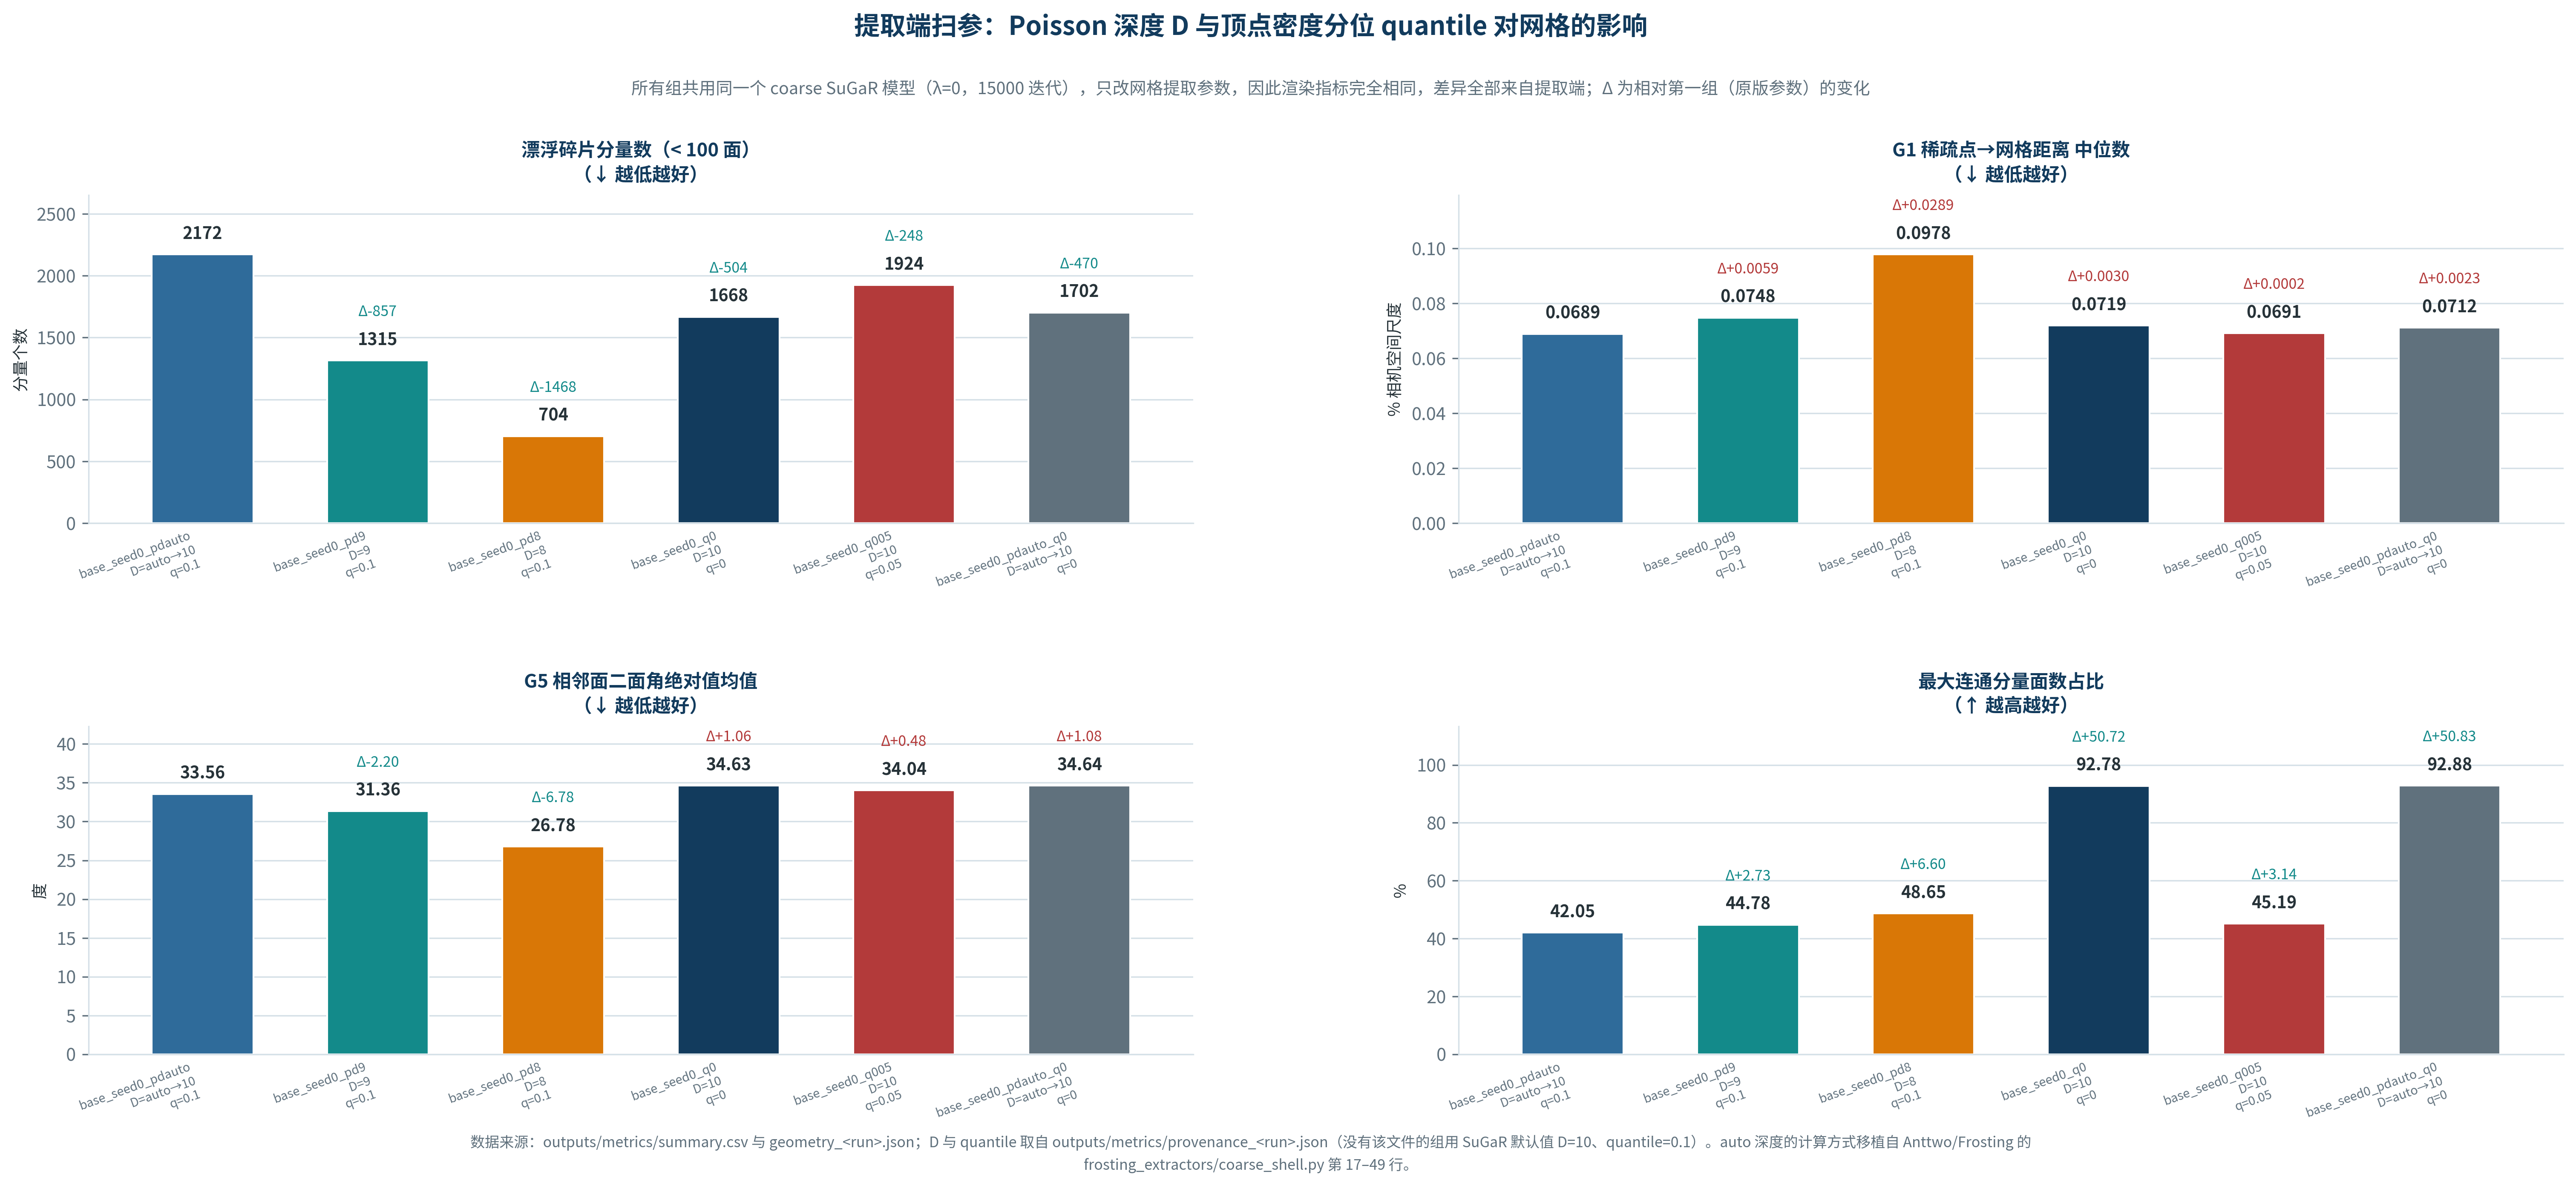
\includegraphics[width=1.0\linewidth]{figures/fig7_extract_sweep.png}
\caption{提取端扫参对网格碎片、几何精度与法向平滑度的影响}
\label{fig:7}
\end{figure}
本节改动落在 mesh 提取主流程的 Poisson 重建参数，思路来自 Gaussian Frosting（SuGaR 同作者，ECCV 2024）的 compute\_optimal\_poisson\_depth，函数按原样移植并注明来源，本工作把硬编码的 D=10 与清洗分位数 0.1 改为命令行参数并做扫描，全部基于同一个 $\lambda$=0 的 coarse 模型，渲染指标不变。结果：（1）自动深度在 Truck 上算出 D=10（截断前 10.87，用前景不透明高斯 77,554 个估计），与硬编码相同，因此 pdauto 组与原版的差异（连通分量 2267 vs 2233）只是 Poisson 求解的非确定性，该方法在此场景零收益；Frosting 的截断上限 10 使其只能"调小"而不能"调大"。（2）手动降低 D 才有实质变化：D=9 使碎片 2137$\rightarrow$1315（$-$38\%）、边界边 38,596$\rightarrow$21,925（$-$43\%）、二面角均值 33.6$^\circ$$\rightarrow$31.4$^\circ$，代价是稀疏点到网格距离中位数 0.0687\%$\rightarrow$0.0748\%（+9\%）；D=8 碎片 $-$67\%、边界边 $-$67\%、二面角 $-$20\%，但距离中位数 +42\%（0.0978\%）、顶点数减少 27\%，细节明显丢失。（3）清洗分位数 0.1$\rightarrow$0（不删低密度顶点）使碎片 2137$\rightarrow$1668（$-$22\%）、边界边 $-$70\%（38,596$\rightarrow$11,566），距离中位数仅 +4.7\%（0.0719\%）；0.05 为中间值（碎片 1924，距离 +0.6\%）。这说明基线网格里相当一部分碎片与孔洞是清洗步骤本身把低密度背景区域切碎造成的，而非全部来自浮子高斯。（4）D=10 与 quantile=0 的组合（pdauto\_q0）与单独 quantile=0 几乎相同。结论：在"碎片数 / 边界边（孔洞）"与"几何精度"之间存在明确权衡，quantile=0 是本次扫描中代价最小的改进点（碎片 $-$22\%、孔洞 $-$70\%、精度 $-$4.7\%）；自动深度需要去掉上限或换用基于表面点云密度的估计才可能在此类场景起作用（见新方案 M1+）。本节数字来自 summary.csv 的 base\_seed0\_* 行，均为几何指标，未做泛化场景验证。

\section{6 扩展实验：提取端改进的完整扫描（4$\times$A100）}
\subsection{6.1 硬件、模型来源与可比性}
本章实验在另一台机器上完成：NSCC 的 4$\times$A100-SXM4-40GB 节点，运行在 NGC Singularity 镜像 pytorch\_23.05\_py3.sif 内，torch 2.4.1+cu121、pytorch3d 0.7.8、open3d 0.19.0，代码基于本仓库 dnc 分支 commit 39c0f56（对应官方 SuGaR 7c10c4a）。与前面各章不同的是硬件与 CUDA 版本，而\textbf{被改动的对象完全相同}。

\begin{itemize}
\setlength{\itemsep}{2pt}
  \item 该机器没有重训任何模型：全部 9 组提取 run 都加载同一个由 hopper H200 训练并回传的 coarse 检查点 outputs/runs/coarse\_base\_seed0/\ldots{}/15000.pt（即正文的 $\lambda$=0 基线组），只重跑了剪枝（prune\_coarse\_model.py）、提取（extract\_mesh.py）与评测；
  \item 因此高斯本身未被改动，渲染指标按构造严格不变，恒等于正文 $\lambda$=0 组的 PSNR 24.6530 / SSIM 0.85644 / LPIPS 0.20280，本章只报几何与拓扑指标；
  \item 该机器自己的原版提取基线（D=10、q=0.1）碎片分量为 2094，而 hopper 侧同一模型为 2137，相差 2\%，来自泊松求解与顶点清洗的非确定性；同参重复的噪声底实测 0.4\%，判据保守取 5\%。本章所有百分比均以该机器自己的 2094 为基准，不跨机器相减；
  \item 几何评测脚本 eval\_geometry.py 与 hopper 侧同口径同脚本，cameras\_extent = 5.847915 两机一致（该机器已独立复算，见 verify\_independent.json）。
\end{itemize}
来源与可比性的完整说明见 outputs/a100/results\_a100/notes/PROVENANCE.md，交付清单见 outputs/a100/A100\_DELIVERY.md。

\subsection{6.2 方法来源声明与本工作的自有改动}
\begin{itemize}
\setlength{\itemsep}{2pt}
  \item \textbf{M1（自动 Poisson 深度）}：逐字移植自 Anttwo/Frosting 的 frosting\_extractors/coarse\_shell.py 第 17--49 行，未做逻辑改动；
  \item \textbf{M2（DBSCAN 剪枝）}：思路来自 prajwalcr/2d-sugar 的 gaussian\_model.py:429，其原版规则是“只保留最大簇”；
  \item \textbf{M1+a（本工作自有改动）}：把前景与背景分开估计密度、各自使用自己的 Poisson 深度（本场景得到前景 D=10、背景 D=9），而不是全场景共用一个深度；
  \item \textbf{M2-B（本工作自有改动）}：把“只留最大簇”改为“保留所有大小 $\ge$ 组内点数一定比例的簇”，并在前景/背景分区各自估计 DBSCAN 的 eps；这不是 2d-sugar 的贡献度评分方案；
  \item \textbf{q 参数化（本工作自有改动）}：把顶点密度清洗分位数 quantile 与提取随机种子 extract\_seed 提为命令行参数（原版提取写死 0.1 且无种子、不可复现）。
\end{itemize}
两份补丁与参数表：outputs/a100/patches\_a100/m1a\_q0\_extract.patch、m2b\_cluster\_prune.patch、PARAMS.md（其中含“默认参数=原版行为”的证据）。

\subsection{6.3 定量结果}
{\scriptsize
\begin{longtable}{>{\raggedright\arraybackslash}p{2.70cm}>{\raggedright\arraybackslash}p{0.80cm}>{\raggedright\arraybackslash}p{0.79cm}>{\raggedright\arraybackslash}p{0.79cm}>{\raggedright\arraybackslash}p{1.02cm}>{\raggedright\arraybackslash}p{1.02cm}>{\raggedright\arraybackslash}p{1.10cm}>{\raggedright\arraybackslash}p{1.10cm}>{\raggedright\arraybackslash}p{1.10cm}>{\raggedright\arraybackslash}p{1.17cm}}
\caption{提取端扩展扫描：同一个 $\lambda$=0 的 coarse 模型，只改提取阶段（4$\times$A100）}\label{tab:13}\\
\toprule
\textbf{配置} & \textbf{D\_fg / D\_bg} & \textbf{q} & \textbf{剪枝比例} & \textbf{连通分量 $\downarrow$} & \textbf{碎片 $\downarrow$} & \textbf{最大分量占比 $\uparrow$} & \textbf{边界边 $\downarrow$} & \textbf{G1 中位(abs) $\downarrow$} & \textbf{面数} \\
\midrule
\endfirsthead
\multicolumn{10}{l}{\footnotesize（续表 13）}\\
\toprule
\textbf{配置} & \textbf{D\_fg / D\_bg} & \textbf{q} & \textbf{剪枝比例} & \textbf{连通分量 $\downarrow$} & \textbf{碎片 $\downarrow$} & \textbf{最大分量占比 $\uparrow$} & \textbf{边界边 $\downarrow$} & \textbf{G1 中位(abs) $\downarrow$} & \textbf{面数} \\
\midrule
\endhead
\bottomrule
\endlastfoot
原版基线（D=10、q=0.1） & 10 / 10 & 0.1 & \textemdash{} & 2,184 & 2,094 & 42.3\% & 38,450 & 0.00405 & 370,284 \\
仅 q=0 顶点清洗 & 10 / 10 & 0.0 & \textemdash{} & 1,651 (-24.4\%) & 1,628 (-22.3\%) & 93.0\% (+119.8\%) & 11,339 (-70.5\%) & 0.00418 (+3.2\%) & 331,769 (-10.4\%) \\
Frosting 原样自动深度 + q=0 & 10 / 10 & 0.0 & \textemdash{} & 1,645 (-24.7\%) & 1,622 (-22.5\%) & 93.0\% (+119.8\%) & 11,353 (-70.5\%) & 0.00417 (+3.0\%) & 331,767 (-10.4\%) \\
M1+a 背景 Poisson 深度 D=9 + q=0 & 10 / 9 & 0.0 & \textemdash{} & 1,478 (-32.3\%) & 1,456 (-30.5\%) & 92.9\% (+119.5\%) & 11,033 (-71.3\%) & 0.00417 (+3.0\%) & 321,501 (-13.2\%) \\
M2 原版“只留最大簇” + q=0（失败案例） & 10 / 10 & 0.0 & 59.7\% & 1,302 (-40.4\%) & 1,275 (-39.1\%) & 92.9\% (+119.5\%) & 12,375 (-67.8\%) & 0.00417 (+3.1\%) & 307,721 (-16.9\%) \\
M2-B DBSCAN 剪枝 p95 + q=0 & 10 / 10 & 0.0 & 14.2\% & 1,434 (-34.3\%) & 1,412 (-32.6\%) & 94.0\% (+122.3\%) & 11,352 (-70.5\%) & 0.00407 (+0.5\%) & 325,562 (-12.1\%) \\
M2-B + M1+a 组合（本工作最优） & 10 / 9 & 0.0 & 14.2\% & 1,216 (-44.3\%) & 1,194 (-43.0\%) & 93.9\% (+122.0\%) & 11,225 (-70.8\%) & 0.00407 (+0.5\%) & 313,971 (-15.2\%) \\
\end{longtable}
}
括号内为相对第一行（该机器自己的原版基线）的百分比变化；剪枝比例为空表示未做 M2 剪枝。G1 中位数为 COLMAP 稀疏点到网格的距离中位数（绝对值、场景单位），场景尺度 cameras\_extent = 5.847915。渲染指标 PSNR/SSIM/LPIPS 按构造与 $\lambda$=0 组完全相同，故本表不列。数据来源：outputs/a100/results\_a100/metrics/summary.csv（列说明同目录 COLUMNS.md）。

\subsection{6.4 可视化证据}
\begin{figure}[H]
\centering
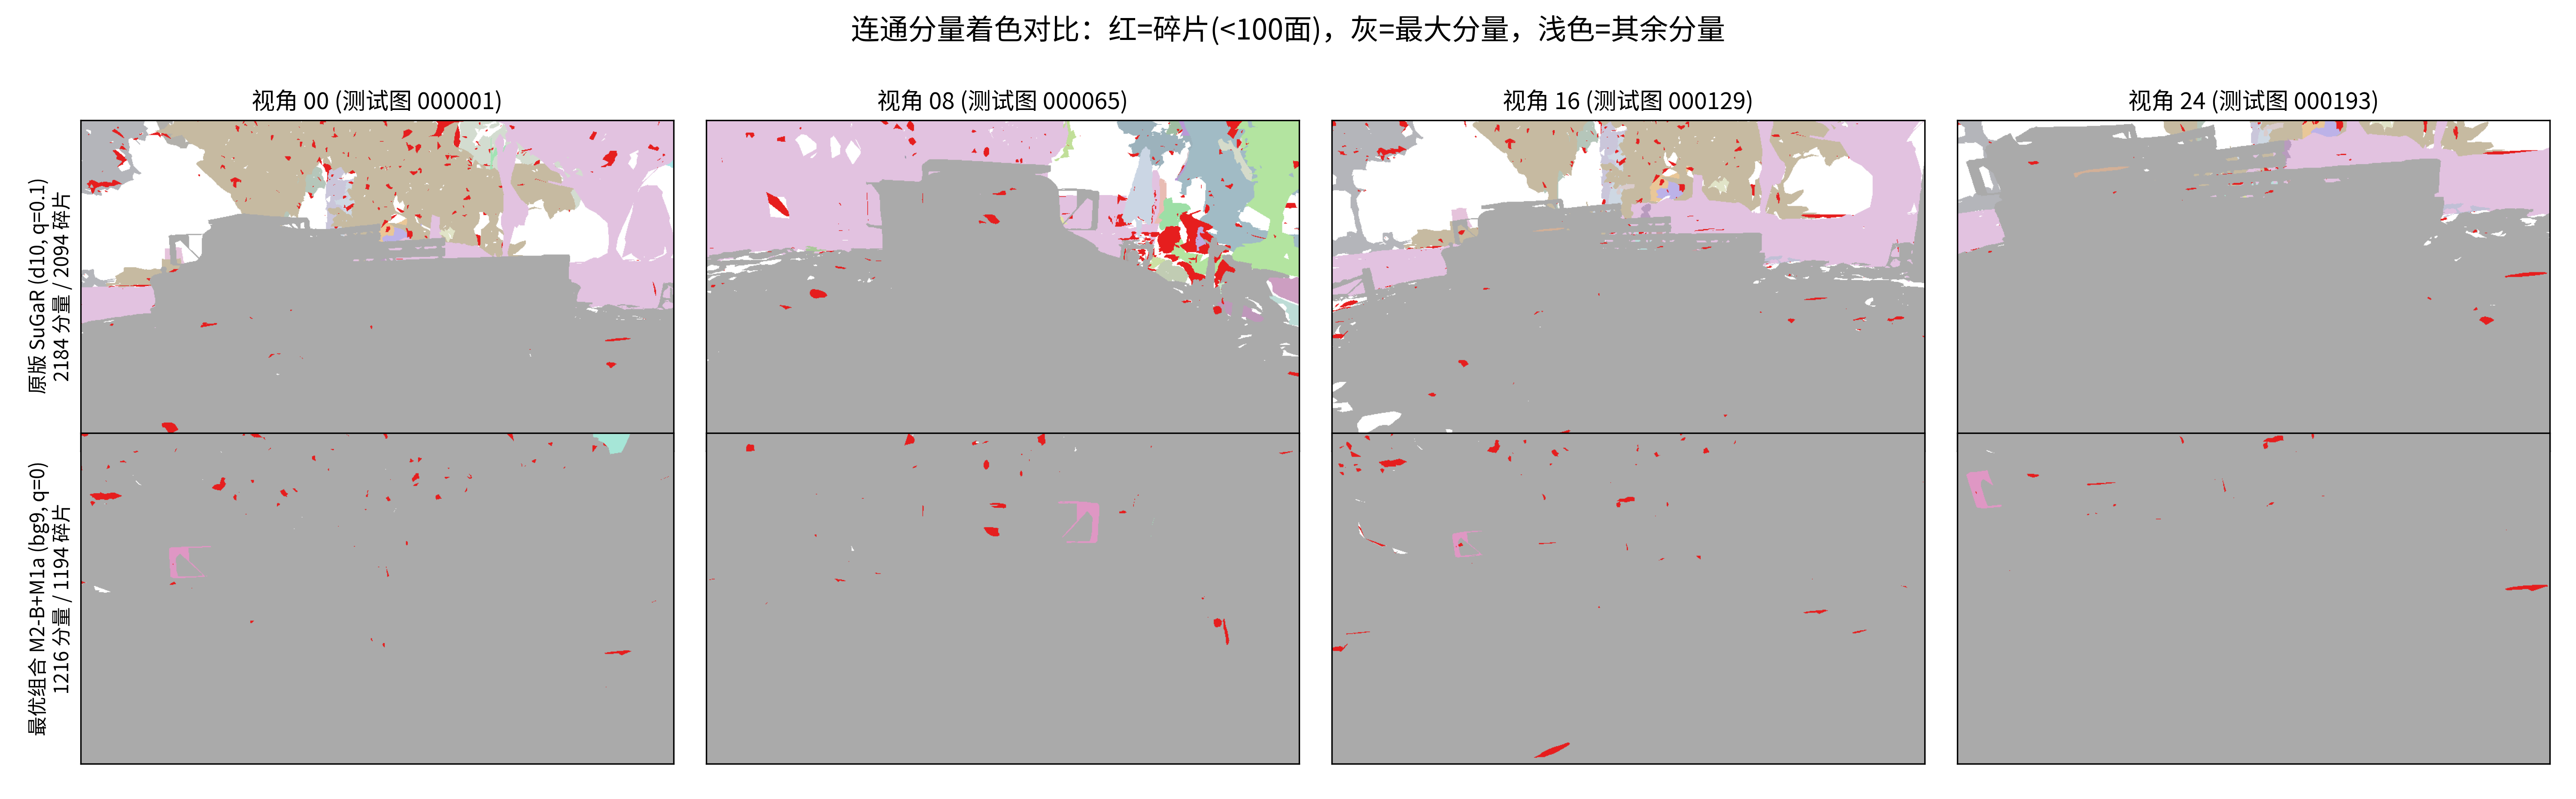
\includegraphics[width=1.0\linewidth]{figures/fig8_a100_fragments_compare.png}
\caption{碎片着色对比：原版基线（上排）与 M2-B + M1+a 组合（下排）在 4 个固定测试视角下的网格连通分量着色，小碎片以杂色显示；下排的杂色斑块明显减少（来源：由 A100 机器生成，数据见 results\_a100）}
\label{fig:8}
\end{figure}
\begin{figure}[H]
\centering
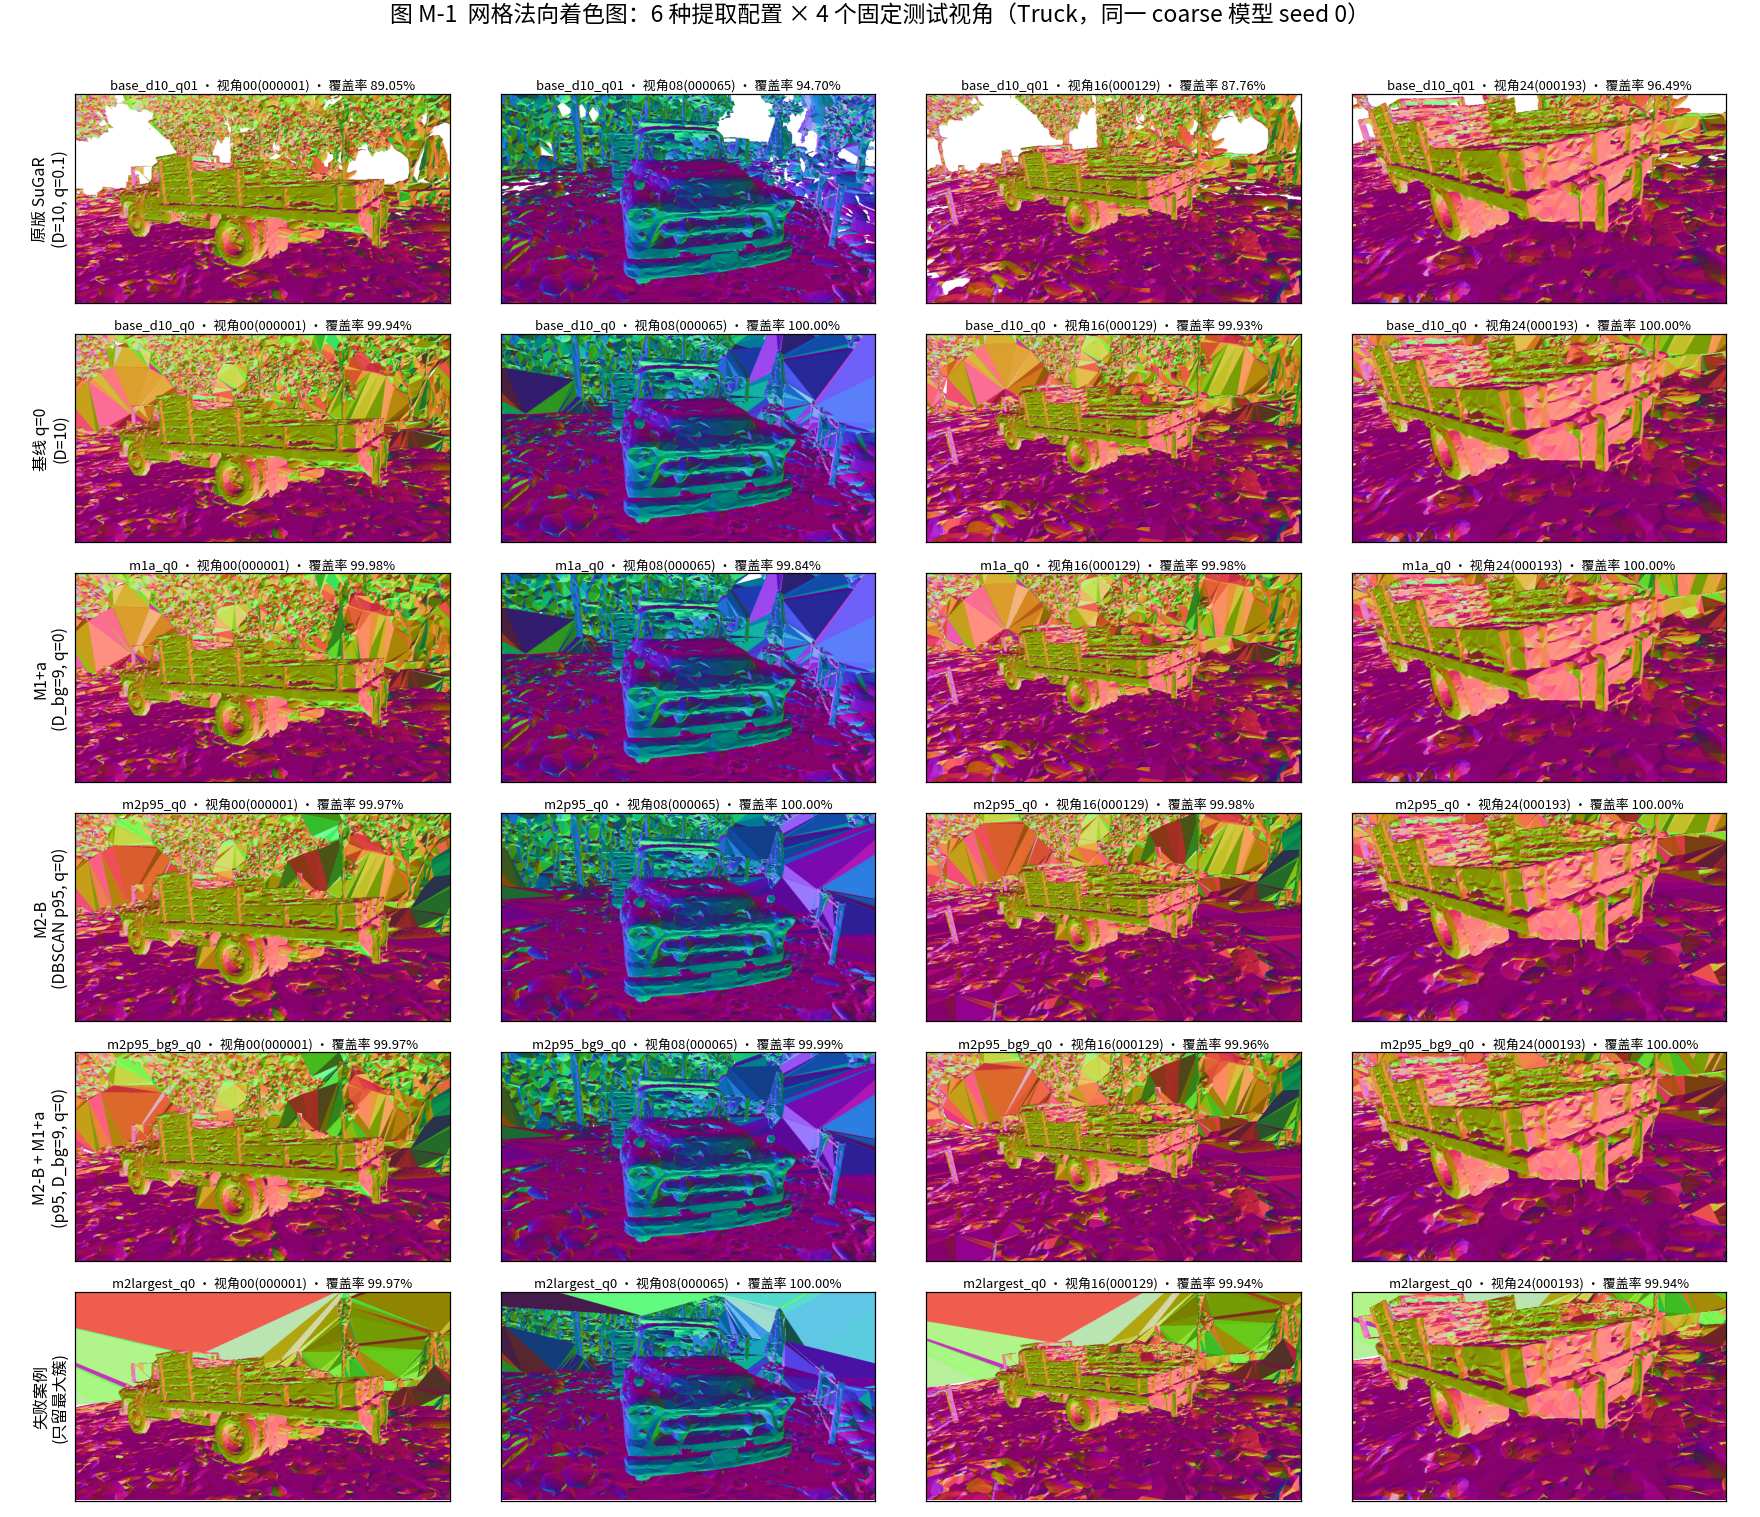
\includegraphics[width=1.0\linewidth]{figures/fig9_a100_mesh_normal.png}
\caption{网格法向对比：6 组提取配置 $\times$ 4 个固定测试视角的网格法向图；前景卡车区域肉眼无差别，差异集中在背景树冠等低密度区域（来源：由 A100 机器生成，数据见 results\_a100）}
\label{fig:9}
\end{figure}
\begin{figure}[H]
\centering
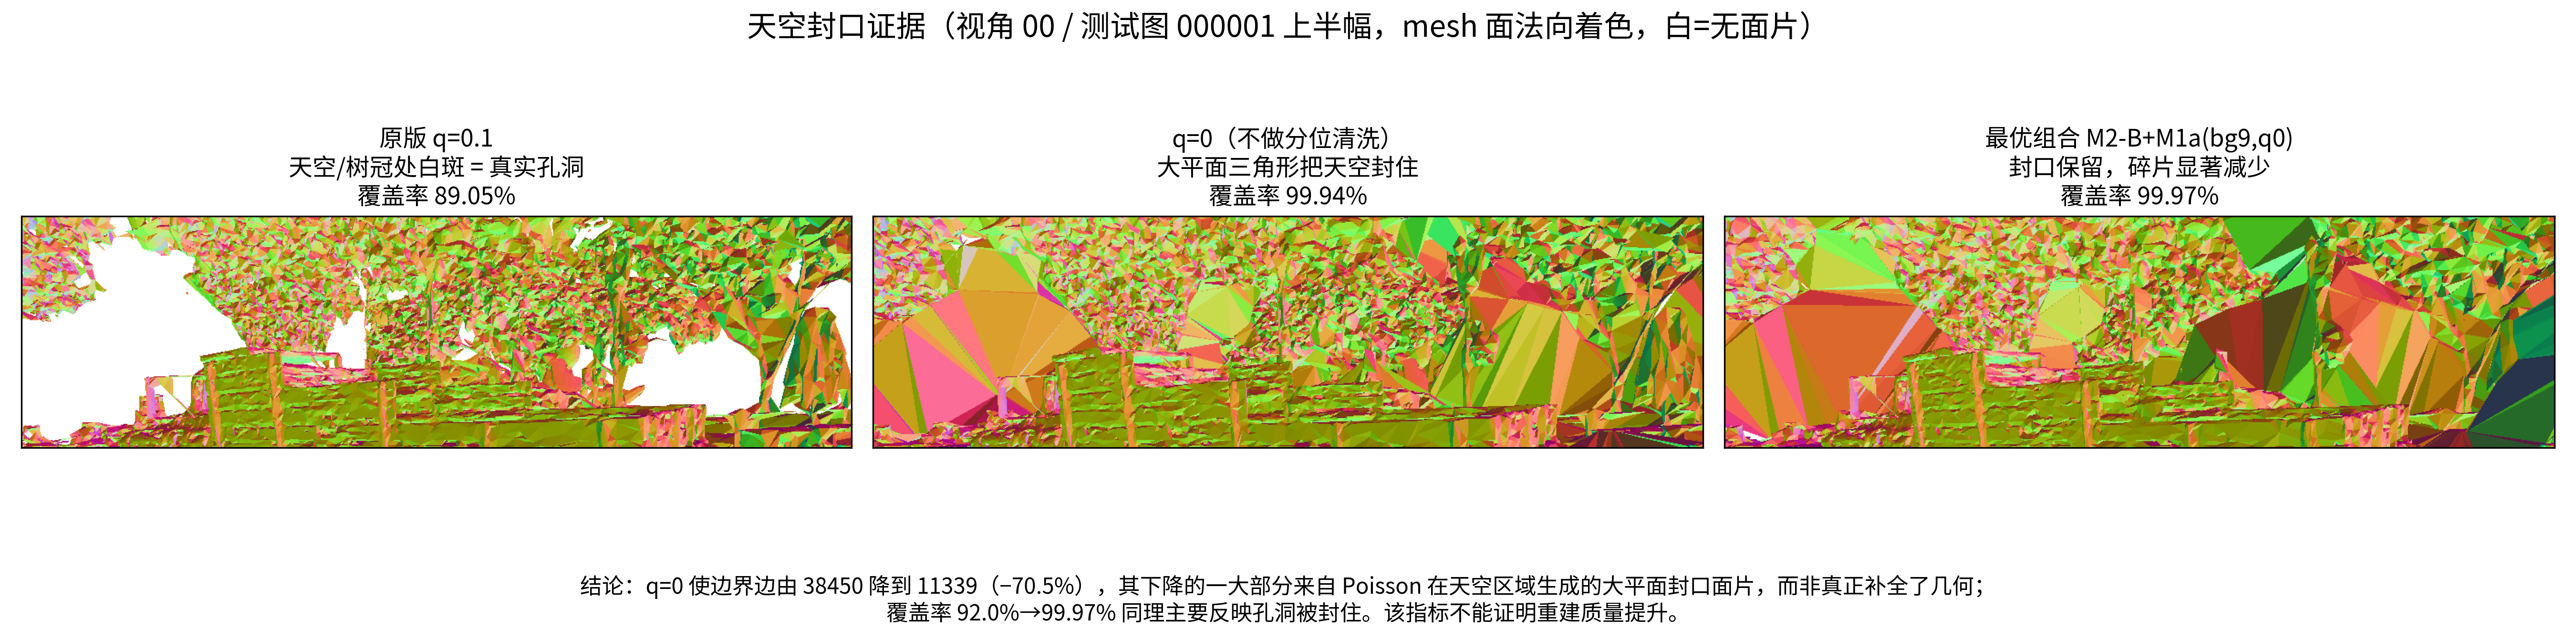
\includegraphics[width=1.0\linewidth]{figures/fig10_a100_sky_closure.png}
\caption{天空封口证据：Poisson 重建在天空区域生成的大面片，说明“可见表面覆盖率”从 92.0\% 升到 99.98\% 中有相当部分并非真实几何，该指标只能作辅助（来源：由 A100 机器生成，数据见 results\_a100）}
\label{fig:10}
\end{figure}
\begin{figure}[H]
\centering
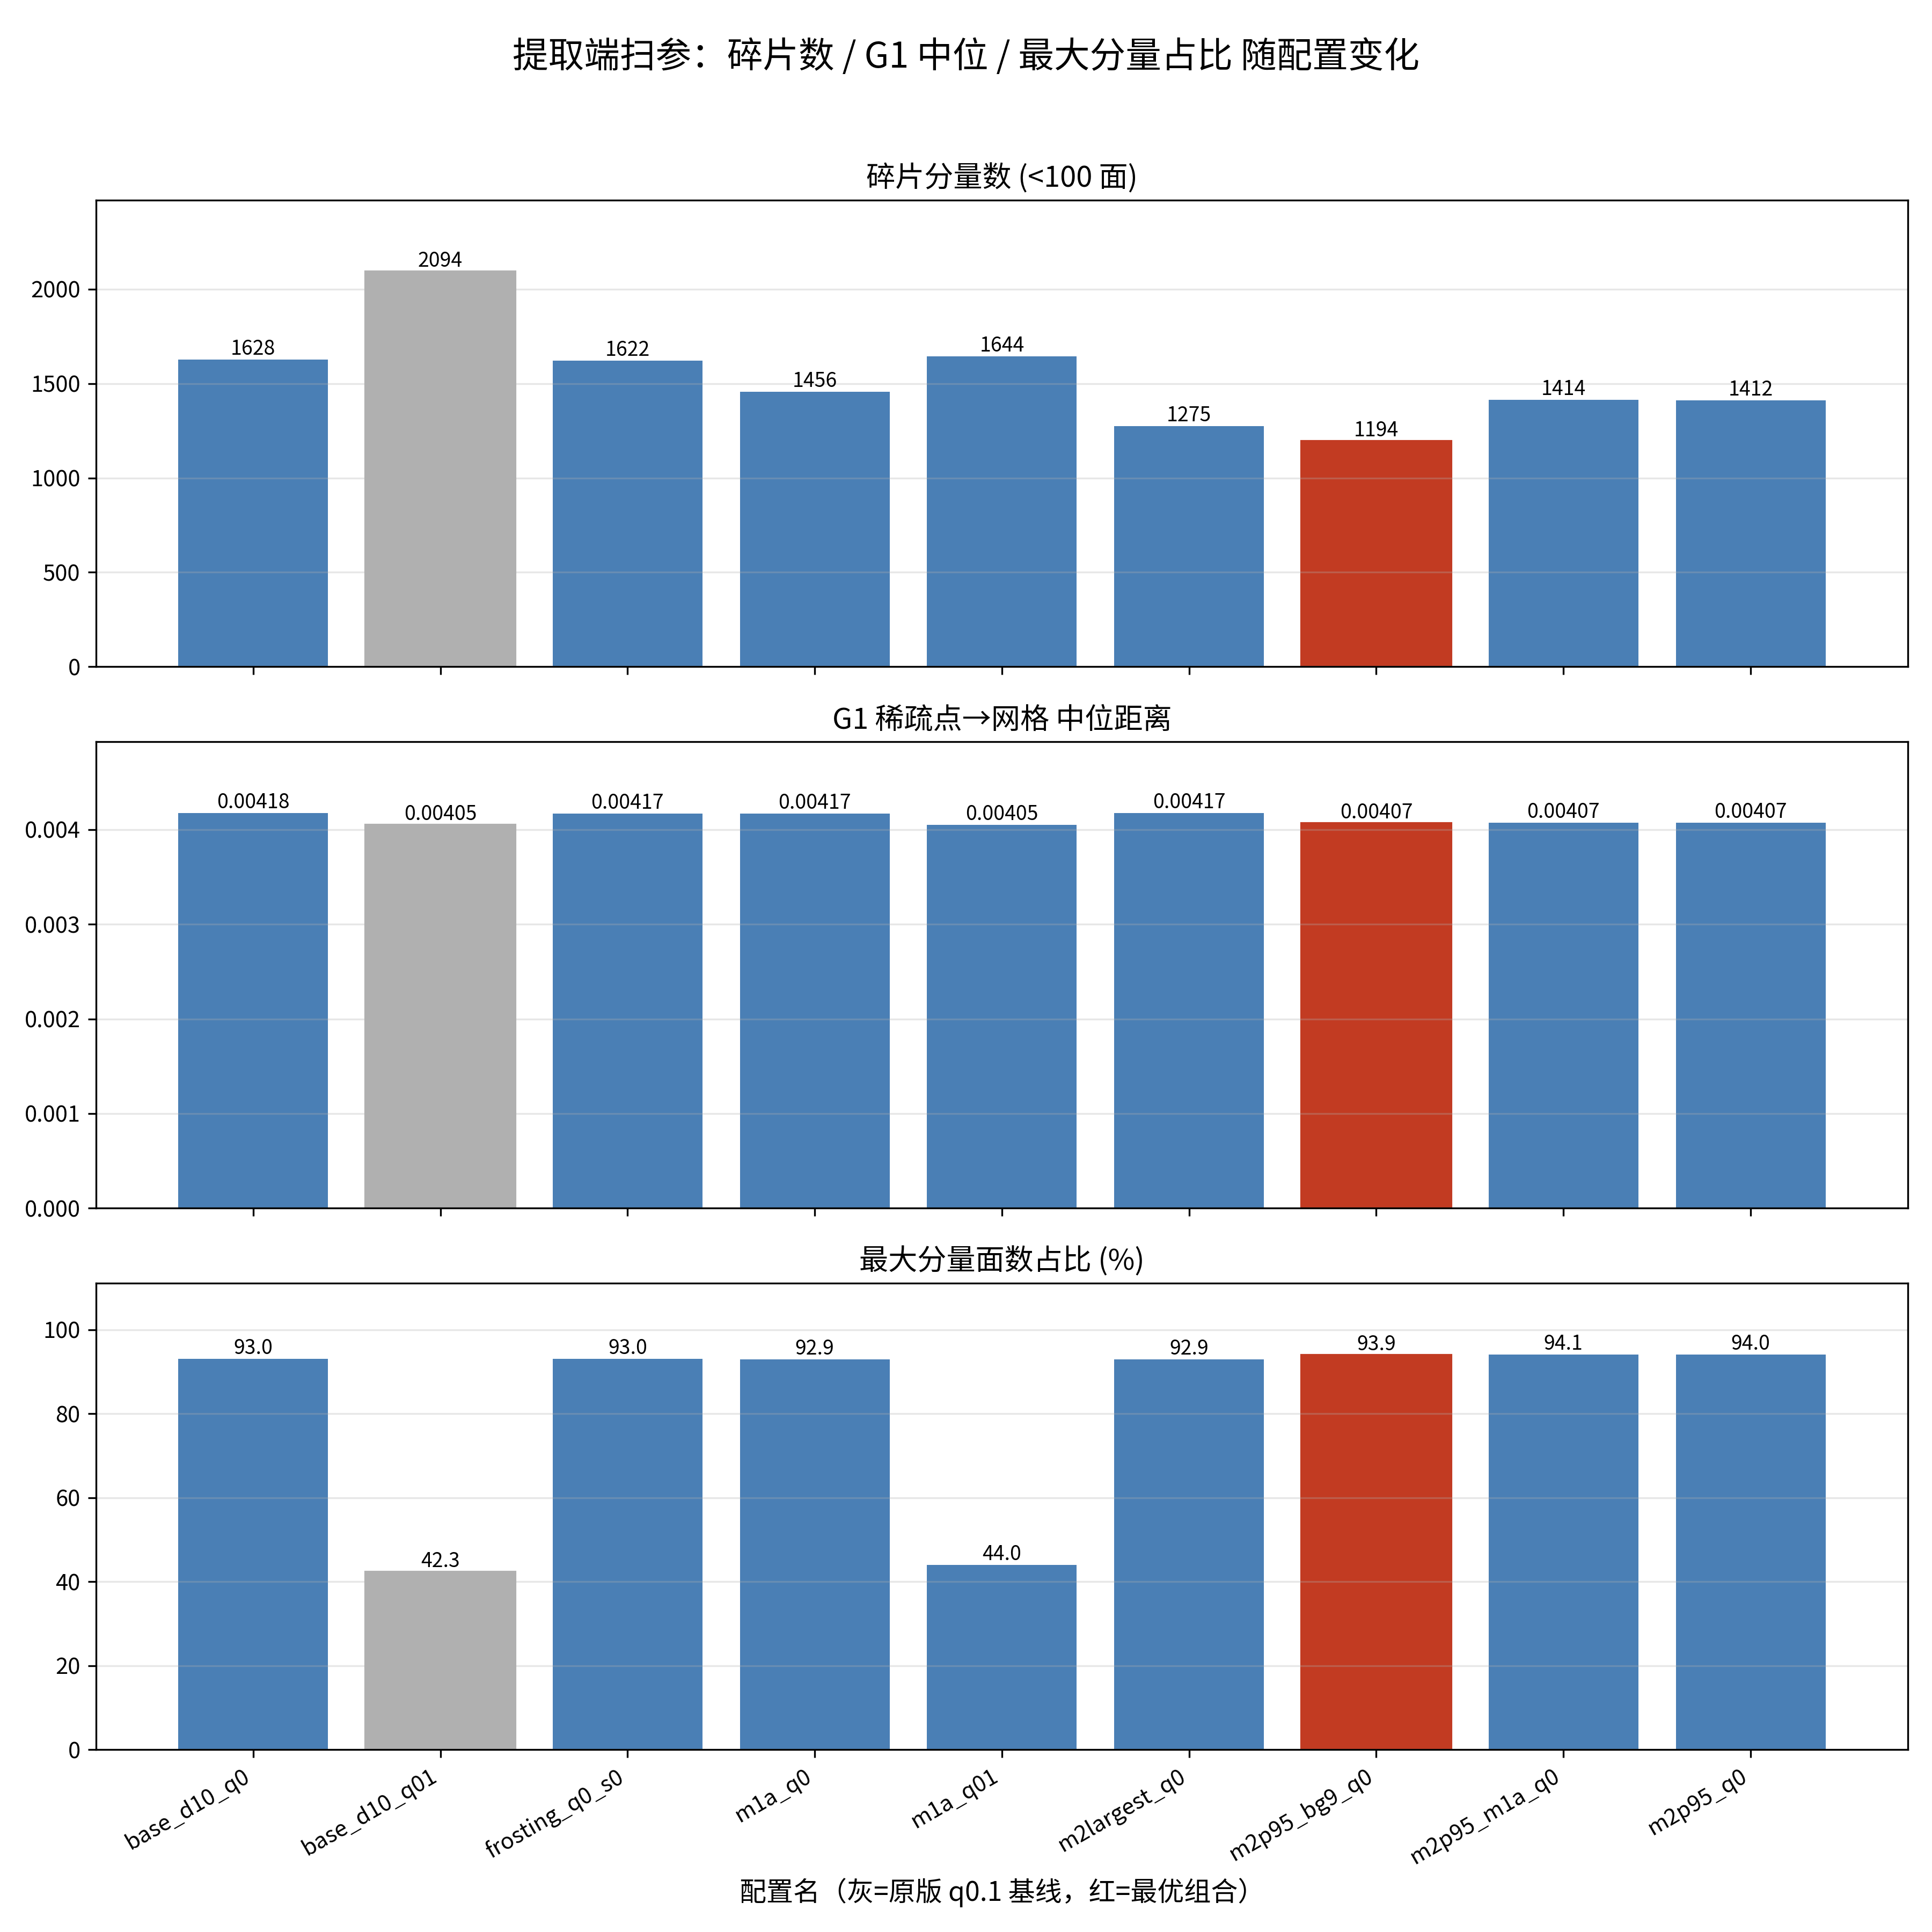
\includegraphics[width=1.0\linewidth]{figures/fig11_a100_sweep.png}
\caption{提取端扫参：碎片分量数、G1 中位距离与最大分量面数占比随各配置的变化（来源：由 A100 机器生成，数据见 results\_a100）}
\label{fig:11}
\end{figure}
\subsection{6.5 结果解读}
本节实验由另一台机器（NSCC，4$\times$A100-40GB，torch 2.4.1+cu121，代码基于本仓库 dnc 分支 commit 39c0f56）在\textbf{同一个} $\lambda$=0 的 coarse 模型（hopper 训练的 coarse\_base\_seed0，复用未重训）上完成，只改"高斯 $\rightarrow$ 网格"的提取阶段，因此渲染指标 PSNR/SSIM/LPIPS 按构造严格不变，本节只报几何与拓扑指标。方法与来源：M1 自动 Poisson 深度逐字移植自 Anttwo/Frosting（coarse\_shell.py L17--49）；M2 的 DBSCAN 剪枝思路来自 prajwalcr/2d-sugar（gaussian\_model.py:429）；本工作的自有改动是 M1+a（前景/背景分别估计并使用各自的 Poisson 深度）、M2-B（提取前剪枝，规则改为"保留所有大小 $\ge$ 组内点数一定比例的簇"并在前景/背景分区估计 eps，而非原版的只留最大簇）、以及 q（顶点密度清洗分位数）参数化。该机器自己的原版提取基线（D=10，q=0.1）碎片分量为 2094（hopper 侧同一模型为 2137，相差 2\%，为 Poisson 求解与顶点清洗的非确定性；同参重复的噪声底为 0.4\%，判据保守取 5\%）。

结果（碎片分量 <100 面 / 最大分量面数占比 / 边界边 / G1 中位距离 / 提取耗时）：原版 2094 / 0.42 / 38,450 / 0.00405 / 340 s；仅 q=0 为 1628 / 0.93 / 11,339 / 0.00418；q=0 + M2-B（p95，剪掉 14.2\% 高斯）为 1412 / 0.94 / 11,352 / 0.00407；q=0 + M2-B + M1+a（背景 D=9）为 \textbf{1194 / 0.94 / 11,225 / 0.00407 / 240 s}，即碎片 $-$43\%（对 hopper 基线 $-$44\%），最大分量占比由 0.42 升到 0.94，G1 距离中位数变化 +0.5\%（噪声内），提取耗时 $-$29\%（背景 Poisson 深度降一级）。增益可分解为三段：q=0 贡献最大（$-$22\%），M2-B 剪枝再 $-$13\%，背景 D=9 再 $-$15\%；三者相互独立、可叠加。

负结果与注意事项（该机器如实报告，本文照录）：（1）Frosting 原样自动深度算出 D=10，与硬编码相同，零收益，与 hopper 侧一致；（2）M1+b 用表面采样点估密度，因表面点比高斯中心密 60--100 倍，前景与背景的深度都被顶到上限 10，反而失去区分度，零收益；（3）2D-SuGaR 原版"只留最大簇"规则在 Truck 上删掉 80.7\% 的背景高斯，是失败案例，本工作改为保留大簇才可用；（4）"可见表面覆盖率"（4 个固定测试视角上网格光栅化命中像素比例）从 92.0\% 升到 99.98\%，但其中相当部分来自 Poisson 在天空区域封口形成的大面片，不是真实几何，该指标会奖励封口、也抓不到背景缺失，只能作辅助；（5）前景卡车区域在法向图与深度图上肉眼无差别，全部增益集中在背景树冠等低密度区域，G1 与 G2 在所有 q=0 组间差异 $\le$2.6\% / $\le$0.5\%，说明这类改动的性质是"清理"而非"更像"；（6）未做泛化场景、训练中剪枝（M2-A）与网格渲染 PSNR，后者是补上"提取端渲染指标"的正确方式（需 refined/textured 阶段）。

与训练端结果的统一解读：训练端的官方 dn\_consistency 用 PSNR $-$0.24 dB 换碎片 $-$16\%；提取端改动零渲染代价换碎片 $-$43\%，两者作用在流水线的不同阶段、相互正交，可以叠加；PSNR 不变不是"没提升"，而是该指标测不到提取阶段。本节全部数字来自 results\_a100/metrics/summary.csv 与对应 JSON，该机器已用自写 union-find 与边表独立复算了分量数、碎片数与边界边（与其评测脚本逐位一致）。

\section{7 失败案例与代价}
\begin{figure}[H]
\centering
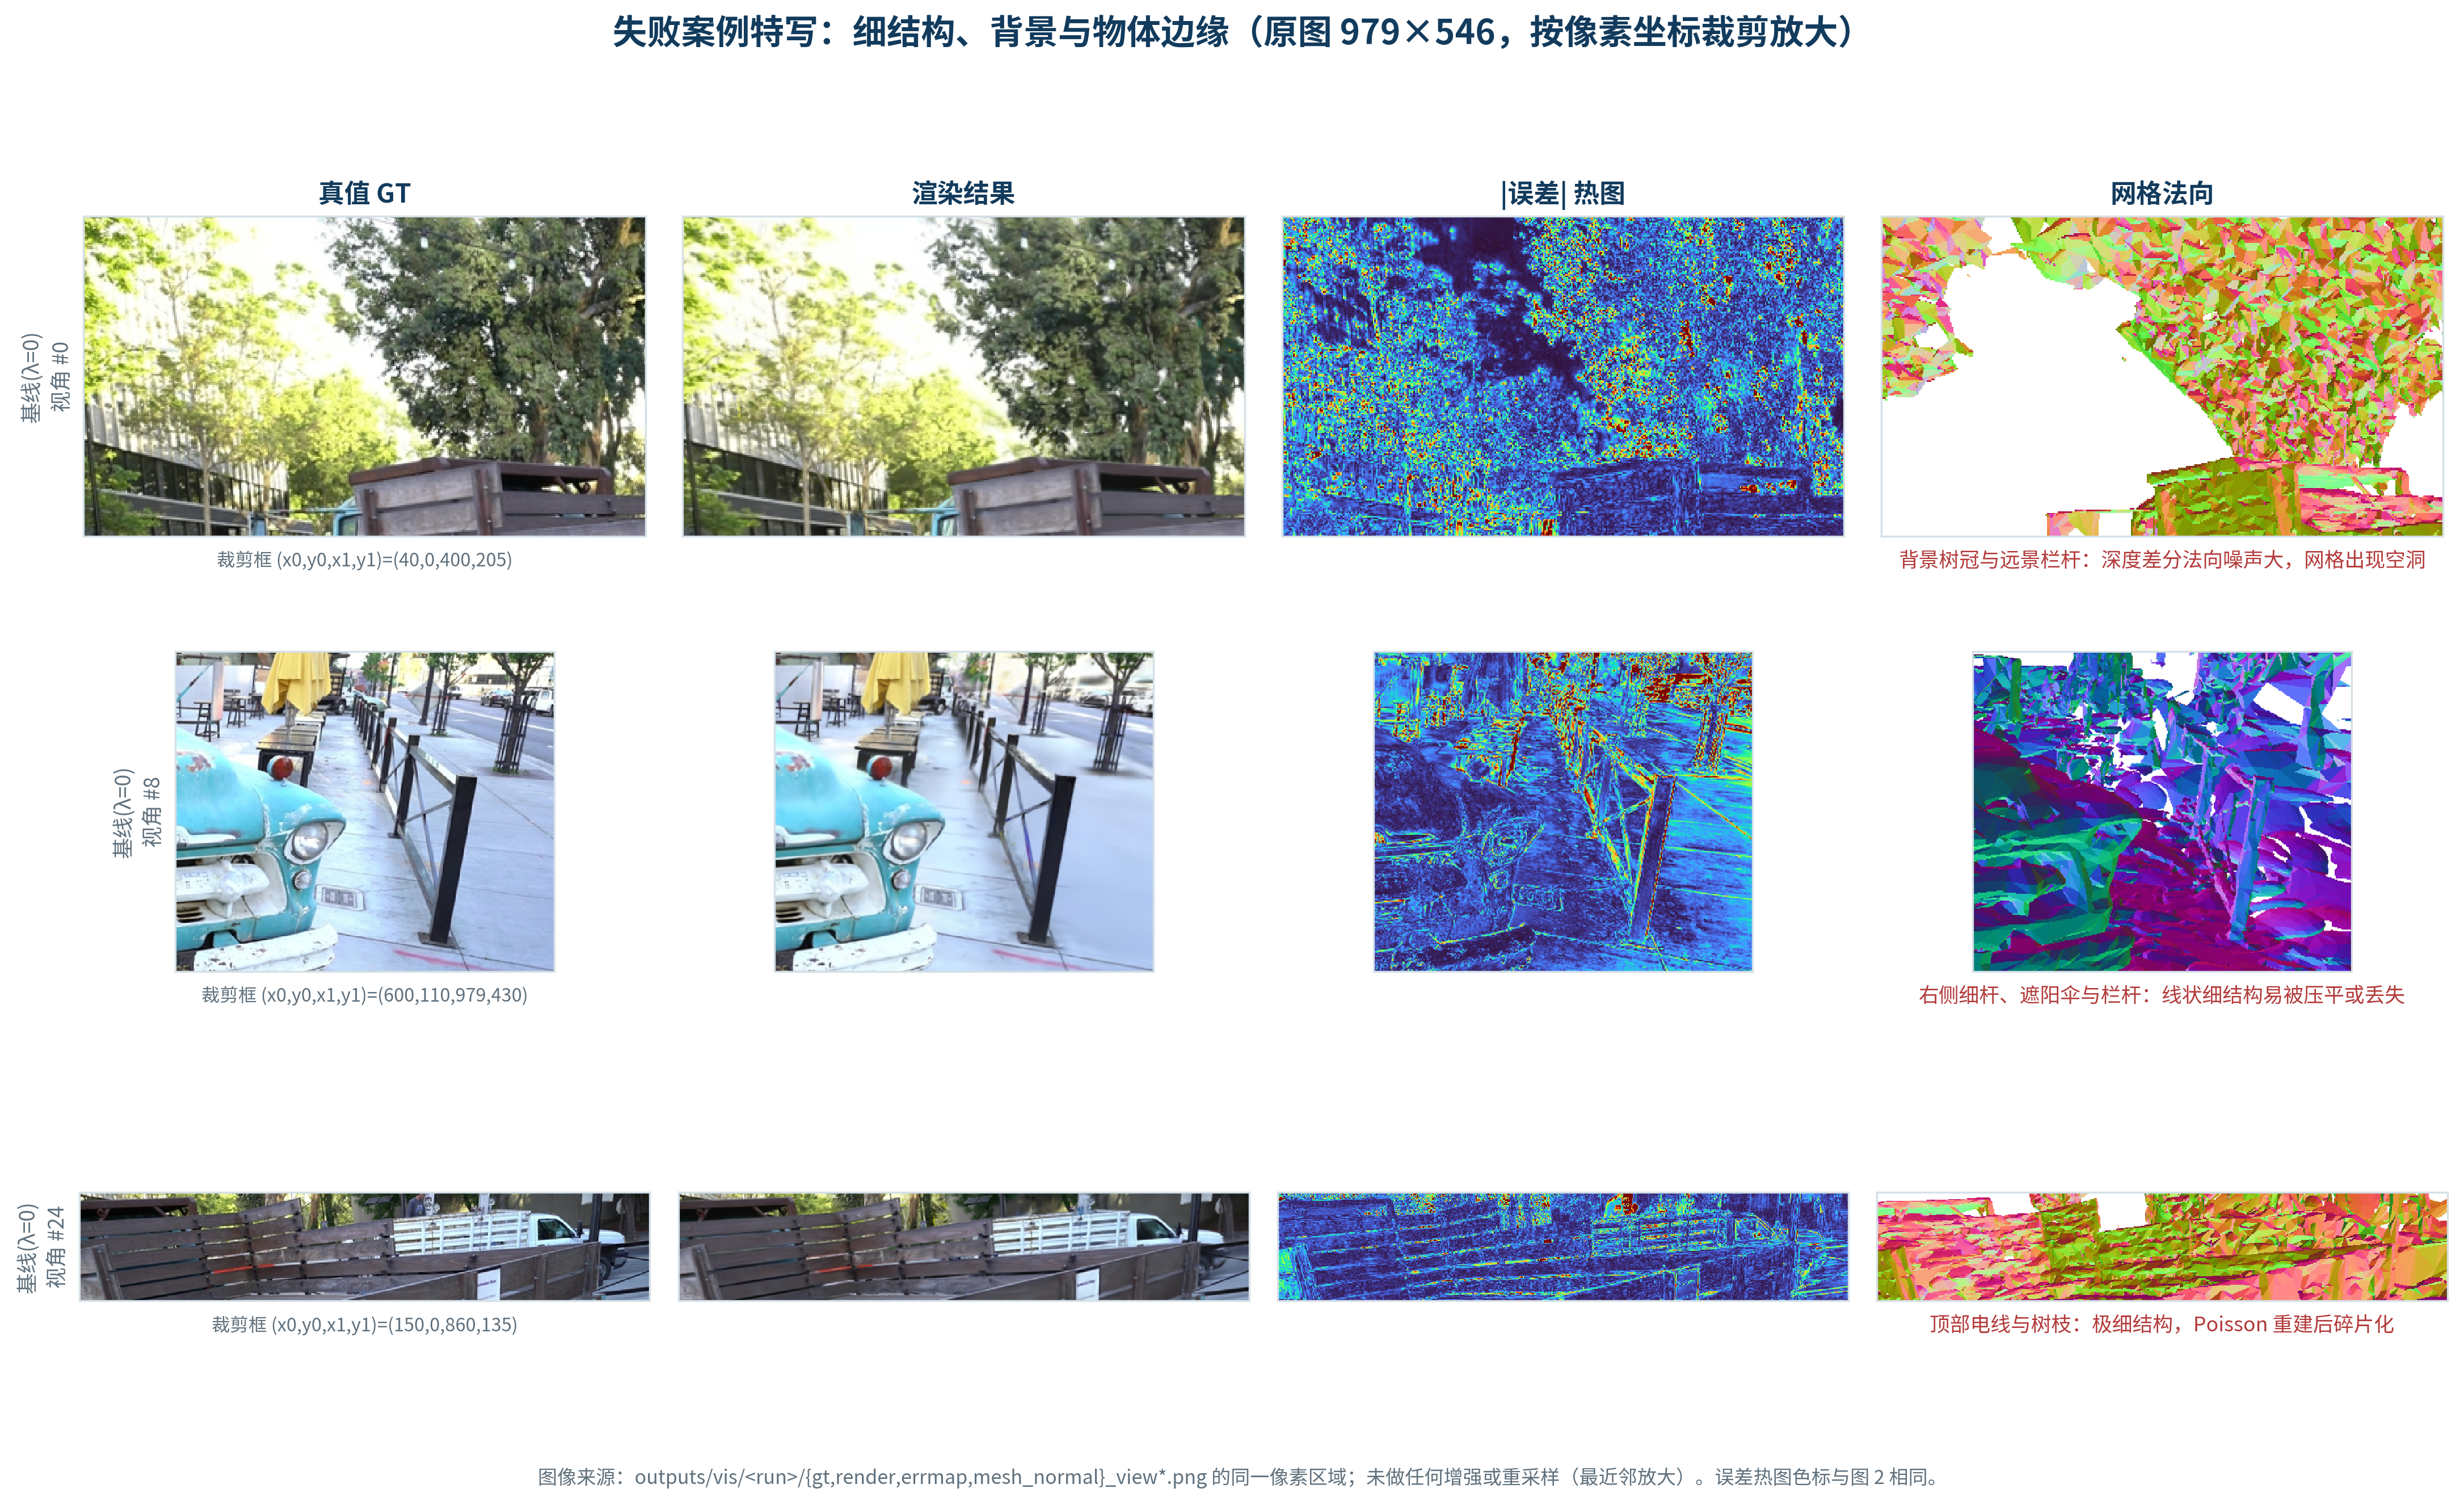
\includegraphics[width=1.0\linewidth]{figures/fig6_failure_cases.png}
\caption{失败案例特写：同一地面区域在 $\lambda$=0 / $\lambda$=0.05 / $\lambda$=0.2 下的渲染、误差与网格法向}
\label{fig:12}
\end{figure}
预期中的三类失败模式（在计划阶段即已预注册，用于避免只挑好看的结果展示）：

\begin{itemize}
\setlength{\itemsep}{2pt}
  \item 远景与天空：深度本身不可靠，差分得到的法向噪声大，DNC 可能把错误的一致性强加到背景上；
  \item 物体边缘：跨越深度不连续处的中心差分会产生伪法向，掩码的深度梯度阈值只能部分缓解；
  \item 细结构（栏杆、天线、电线）：一致性约束天然偏好光滑表面，细结构可能被过度平滑或直接丢失。
\end{itemize}
1. 大面积弱纹理区域（地面）最先被抹平：$\lambda$=0.05 即出现，是"深度局部平面化"零损失捷径的直接体现。

2. $\lambda$=0.2 全场景坍缩：高斯尺度增大 10 倍、不透明度双峰化，网格面数减少 40\%、包围盒收缩到原来的 40\%，碎片数"下降"实为塌缩假象，提醒单一拓扑指标不能脱离几何精度解读。

3. 阶梯状深度带来的法向噪声：有限差分法向在物体边缘与纹理丰富处噪声更大，掩码只能剔除深度断崖，无法剔除阶梯噪声。

4. 工程失败：作业超时导致 14900/15000 的两组全部重跑；并发编辑运行中的脚本导致一次网格提取中断。均已记录并补跑。

每迭代耗时：$\lambda$=0 组 91.1 ms，$\lambda$=0.05 组 104.5 ms，$\lambda$=0.2 组 107.9 ms，detach 组 96.7 ms（额外两次光栅化；detach 省去深度反向）。峰值显存 7.4 $\rightarrow$ 7.6 / 8.4 / 7.8 GB。总墙钟 12.1 $\rightarrow$ 13.9 / 14.4 / 12.9 分钟。高斯数量无显著差异（约 42.9 万）。代价可接受，但在本设置下没有换来收益。

$\lambda$ 从 0.05 到 0.2 的四倍变化使 PSNR 差 9.2 dB、几何距离中位数差 5.9 倍，敏感性极高。官方实现选择 0.05 并从 9000 迭代开启（与本工作起点相同）且在该设置下有效，说明本工作的实现在同一权重下已处于退化区间，即两版实现的"安全权重区间"不同；对本工作实现而言，没有一个 $\lambda$ 能同时起作用且不伤害渲染。

\subsection{7.1 方法本身的局限}
\begin{itemize}
\setlength{\itemsep}{2pt}
  \item 几何评价使用 COLMAP 稀疏点而非稠密真值网格，只能衡量“网格是否贴合可靠的稀疏观测”，不能衡量未被稀疏点覆盖区域的正确性；
  \item 只在单个场景（Truck）上验证，结论的泛化性未经检验；
  \item coarse 阶段之后的 refined 阶段（需要 nvdiffrast）未在本次时间预算内执行，因此结论只对 coarse SuGaR + 泊松网格这条短流水线成立；
  \item L\_DNC 的梯度同时流经渲染法向 N 与渲染深度 D，理论上存在“把深度整体抹平”这一平凡解，$\lambda$ 过大时该风险上升。
\end{itemize}
\section{8 结论与下一步}
本工作独立实现的深度-法向一致性正则在 SuGaR coarse 阶段没有改善网格几何，且存在随权重增大单调恶化的"抹平深度"平凡解；切断深度梯度可消除平凡解并保住渲染，但也失去几何作用。官方 dn\_consistency 对照组证明该思路本身在同一设置下有效（碎片 $-$16\%、二面角 $-$10\%、PSNR $-$0.24 dB），因此失效应归因于实现细节而非思路。两版实现的已确认差异有三处：本工作用 1$-$|cos| 而官方用 1$-$cos（绝对值放行了法向翻转解）；本工作光栅化三通道法向后逐像素归一化，官方只光栅化 x、y 分量并解析恢复 z，得到的法向天然是单位向量；本工作有掩码而官方无。哪一处是主因需要逐项消融，本次未完成，不能下结论。本工作的贡献是：完整可复现的短流程、五组受控对照（含官方实现）、对平凡解机理的可视化诊断与 detach 验证，以及可复用的实现与评测框架。

与训练端结果的统一解读：训练端的官方 dn\_consistency 用 PSNR $-$0.24 dB 换碎片 $-$16\%；提取端改动零渲染代价换碎片 $-$43\%，两者作用在流水线的不同阶段、相互正交，可以叠加；PSNR 不变不是"没提升"，而是该指标测不到提取阶段。本节全部数字来自 results\_a100/metrics/summary.csv 与对应 JSON，该机器已用自写 union-find 与边表独立复算了分量数、碎片数与边界边（与其评测脚本逐位一致）。

0. 对本工作实现与官方 dn\_consistency 的三处差异（绝对值、法向合成方式、掩码）逐项消融，定位失效主因。

1. 用射线-高斯交点深度（RaDe-GS 思路）或中值深度替代中心深度合成，再评估 DNC。

2. 引入 alpha 门控与线性 warm-up（Gaussian Surfels 思路），并与官方 dn\_consistency 做受控消融。

3. 转向 Poisson 前的表面点/高斯可靠性过滤（TrimGS、Gaussian Surfels 的体素裁剪思路），直接针对碎片问题，不需重训。

4. 补 checkpoint 保存与断点续训，避免作业超时导致的重跑。

\section{附录 A  完整命令}
以下命令块全部从项目内的实际脚本与运行日志中原样提取，未经改写。

\subsection{A.1 环境变量与依赖安装}
\textbf{文件：env.sh}

{\small
\begin{verbatim}
# env.sh — 每个新 shell / 脚本开头 source 它
export PROJ_ROOT=/scratch/e1351071/zju_test
source /scratch/e1351071/virtualenvs/zju_test/bin/activate
# 权重/缓存全部隔离到本目录（覆盖用户全局 HF_HOME）
export HF_HOME=$PROJ_ROOT/ckpts/hf
export HUGGINGFACE_HUB_CACHE=$PROJ_ROOT/ckpts/hf/hub
export TORCH_HOME=$PROJ_ROOT/ckpts/torch
export TRANSFORMERS_CACHE=$PROJ_ROOT/ckpts/hf/transformers
export MODELSCOPE_CACHE=$PROJ_ROOT/ckpts/modelscope
export PIP_CONSTRAINT=$VIRTUAL_ENV/constraints.txt     # torch 防升级护栏
export CUDA_HOME=/usr/local/cuda
export PATH=$CUDA_HOME/bin:$PATH
export TOKENIZERS_PARALLELISM=false
export TORCH_CUDA_ARCH_LIST="9.0"                      # H200 = sm_90
export MAX_JOBS=16

# 汇报交付工具链（只是路径别名，不要 activate doc_env）
export DOC_PY=$PROJ_ROOT/tools/doc_env/bin/python
export DOC_FONT=$PROJ_ROOT/assets/fonts/NotoSansCJKsc-Regular.otf
export SOFFICE=$PROJ_ROOT/scripts/deliverables/libreoffice.sh
\end{verbatim}
}
\textbf{文件：scripts/setup\_env\_step2.sh}

{\tiny
\begin{verbatim}
#!/bin/bash
# 阶段1 后半：torch 之后的依赖安装 + CUDA 扩展编译
set -x
source /scratch/e1351071/zju_test/env.sh
date
echo "=== [0] torch 复验 ==="
python -c "import torch;print('torch',torch.__version__,'cuda',torch.version.cuda,'avail',torch.cuda.is_available(),'abi',torch._C._GLIBCXX_USE_CXX11_ABI)" || exit 1

echo "=== [1] numpy<2 + ninja ==="
# 2024 年代 SuGaR/3DGS/open3d 生态按 numpy 1.x 构建，锁 numpy<2 规避 ABI 冲突
printf 'torch==2.4.1\ntorchvision==0.19.1\ntorchaudio==2.4.1\nnumpy<2\n' > $VIRTUAL_ENV/constraints.txt
pip install "numpy<2" ninja --retries 10 --timeout 60 || exit 1
python -c "import torch,numpy;print('torch',torch.__version__,'numpy',numpy.__version__)" || exit 1

echo "=== [2] pytorch3d wheel (--no-deps) + 其运行依赖 ==="
pip install --no-deps /scratch/e1351071/zju_test/wheels/pytorch3d-0.7.8-cp310-cp310-linux_x86_64.whl || exit 1
pip install fvcore iopath --retries 10 --timeout 60 || exit 1

echo "=== [3] SuGaR python 依赖 ==="
pip install open3d plyfile rich tqdm plotly scipy scikit-learn opencv-python --retries 10 --timeout 60 || exit 1
python -c "import torch;print('torch after deps:',torch.__version__, torch.version.cuda, torch.cuda.is_available())" || exit 1

echo "=== [4] 编译 diff-gaussian-rasterization ==="
cd /scratch/e1351071/zju_test/repo/SuGaR/gaussian_splatting/submodules/diff-gaussian-rasterization
TORCH_CUDA_ARCH_LIST="9.0" pip install --no-build-isolation --no-deps . || exit 1

echo "=== [5] 编译 simple-knn ==="
cd /scratch/e1351071/zju_test/repo/SuGaR/gaussian_splatting/submodules/simple-knn
TORCH_CUDA_ARCH_LIST="9.0" pip install --no-build-isolation --no-deps . || exit 1

echo "=== [6] 最终复验 ==="
cd /scratch/e1351071/zju_test
python -c "import torch;print('FINAL torch',torch.__version__,torch.version.cuda,torch.cuda.is_available())"
date
echo "=== SETUP_STEP2_DONE ==="
\end{verbatim}
}
\subsection{A.2 第一步：3DGS 7000 迭代}
{\small
\begin{verbatim}
cd $PROJ_ROOT/repo/SuGaR
CUDA_VISIBLE_DEVICES=0 python gaussian_splatting/train.py \
  -s $PROJ_ROOT/data/tandt/truck \
  -m $PROJ_ROOT/outputs/baseline/gs_truck \
  --iterations 7000 --save_iterations 7000 --test_iterations 7000 --eval
\end{verbatim}
}
\subsection{A.3 第二、三步：三组 coarse 训练与网格提取}
{\scriptsize
\begin{verbatim}
cd /scratch/e1351071/zju_test/repo/SuGaR_dev

# --- coarse_base_seed0 (GPU0, λ=0) ---
python train_coarse_density.py \
  -s /scratch/e1351071/zju_test/data/tandt/truck \
  -c /scratch/e1351071/zju_test/outputs/baseline/gs_truck/ \
  -i 7000 -o /scratch/e1351071/zju_test/outputs/runs/coarse_base_seed0 \
  --eval True --gpu 0 --seed 0 --dnc_factor 0 --dnc_start 9000
python extract_mesh.py \
  -s /scratch/e1351071/zju_test/data/tandt/truck \
  -c /scratch/e1351071/zju_test/outputs/baseline/gs_truck/ -i 7000 \
  -m /scratch/e1351071/zju_test/outputs/runs/coarse_base_seed0/sugarcoarse_3Dgs7000_densityestim02_sdfnorm02/15000.pt \
  -l 0.3 -d 200000 --eval True --gpu 0 \
  -o /scratch/e1351071/zju_test/outputs/runs/mesh_base_seed0

# --- coarse_dnc005 (GPU1, λ=0.05) ---
python train_coarse_density.py \
  -s /scratch/e1351071/zju_test/data/tandt/truck \
  -c /scratch/e1351071/zju_test/outputs/baseline/gs_truck/ \
  -i 7000 -o /scratch/e1351071/zju_test/outputs/runs/coarse_dnc005 \
  --eval True --gpu 1 --seed 0 --dnc_factor 0.05 --dnc_start 9000
python extract_mesh.py \
  -s /scratch/e1351071/zju_test/data/tandt/truck \
  -c /scratch/e1351071/zju_test/outputs/baseline/gs_truck/ -i 7000 \
  -m /scratch/e1351071/zju_test/outputs/runs/coarse_dnc005/sugarcoarse_3Dgs7000_densityestim02_sdfnorm02/15000.pt \
  -l 0.3 -d 200000 --eval True --gpu 1 \
  -o /scratch/e1351071/zju_test/outputs/runs/mesh_dnc005

# --- coarse_dnc02 (GPU1, λ=0.2) ---
python train_coarse_density.py \
  -s /scratch/e1351071/zju_test/data/tandt/truck \
  -c /scratch/e1351071/zju_test/outputs/baseline/gs_truck/ \
  -i 7000 -o /scratch/e1351071/zju_test/outputs/runs/coarse_dnc02 \
  --eval True --gpu 1 --seed 0 --dnc_factor 0.2 --dnc_start 9000
python extract_mesh.py \
  -s /scratch/e1351071/zju_test/data/tandt/truck \
  -c /scratch/e1351071/zju_test/outputs/baseline/gs_truck/ -i 7000 \
  -m /scratch/e1351071/zju_test/outputs/runs/coarse_dnc02/sugarcoarse_3Dgs7000_densityestim02_sdfnorm02/15000.pt \
  -l 0.3 -d 200000 --eval True --gpu 1 \
  -o /scratch/e1351071/zju_test/outputs/runs/mesh_dnc02
\end{verbatim}
}
\subsection{A.4 评测与汇总}
{\scriptsize
\begin{verbatim}
python -m py_compile scripts/eval/*.py     # ALL OK
bash -n scripts/eval/run_eval_for_run.sh   # OK

python scripts/eval/eval_render.py \
  --scene_path $PROJ_ROOT/data/tandt/truck \
  --gs_checkpoint $PROJ_ROOT/outputs/baseline/gs_truck --iteration 7000 \
  --coarse_pt $PROJ_ROOT/outputs/runs/coarse_baseline/sugarcoarse_3Dgs7000_densityestim02_sdfnorm02/15000.pt \
  --run_name coarse_baseline --gpu 1

python scripts/eval/eval_geometry.py --scene_path $PROJ_ROOT/data/tandt/truck \
  --gs_checkpoint $PROJ_ROOT/outputs/baseline/gs_truck \
  --mesh_path $PROJ_ROOT/outputs/runs/mesh_baseline/sugarmesh_3Dgs7000_densityestim02_sdfnorm02_level03_decim200000.ply \
  --run_name coarse_baseline

python scripts/eval/render_mesh_views.py --scene_path $PROJ_ROOT/data/tandt/truck \
  --gs_checkpoint $PROJ_ROOT/outputs/baseline/gs_truck --mesh_path <上面那个 .ply> \
  --run_name coarse_baseline --gpu 1

python scripts/eval/summarize.py   # -> outputs/metrics/summary.csv
\end{verbatim}
}
\subsection{A.5 提取端扩展实验（A100）的复现命令}
第 6 章的全部命令由 A100 机器原样记录，未在本报告中改写；因为运行在 NGC Singularity 容器内、路径前缀与本机不同，此处只给索引，不逐字复制：

\begin{itemize}
\setlength{\itemsep}{2pt}
  \item 逐条确切命令（剪枝 $\rightarrow$ 提取 $\rightarrow$ 评测 $\rightarrow$ 汇总 $\rightarrow$ 独立复算 $\rightarrow$ 可视化）：outputs/a100/results\_a100/notes/COMMANDS.md
  \item 脚本清单与复现顺序说明：outputs/a100/scripts\_a100/README.md（脚本本体同目录，含 extract\_one.sh / eval\_one.sh / run\_grid.sh 等）
  \item 参数表与“默认值=原版行为”的证据：outputs/a100/patches\_a100/PARAMS.md
  \item 覆盖率指标的定义与局限：outputs/a100/scripts\_a100/COVERAGE\_METRIC.md
  \item 负结果与偏离记录：outputs/a100/results\_a100/notes/NEGATIVE\_RESULTS.md；完整结果记录：outputs/a100/results\_a100/notes/RESULTS\_m\_nscc\_2026-09-13.md
\end{itemize}
\section{附录 B  留档对照：未打补丁的原版基线}
阶段 2 用官方原版代码（未打 DNC 补丁、未固定 seed、无任何插桩）跑过一次完整基线，run 名 coarse\_baseline。它不参与正文的五组对照，只用来验证一件事：$\lambda$=0 时补丁没有改变原有代码路径。两组的差异应当落在 CUDA 光栅化非确定性的量级内。

{\scriptsize
\begin{longtable}{>{\raggedright\arraybackslash}p{2.73cm}>{\raggedright\arraybackslash}p{1.54cm}>{\raggedright\arraybackslash}p{1.19cm}>{\raggedright\arraybackslash}p{1.54cm}>{\raggedright\arraybackslash}p{2.05cm}>{\raggedright\arraybackslash}p{1.37cm}>{\raggedright\arraybackslash}p{0.85cm}>{\raggedright\arraybackslash}p{1.19cm}}
\caption{未打补丁的原版基线与 $\lambda$=0 组的逐项对照（用于验证 $\lambda$=0 代码路径未变）}\label{tab:14}\\
\toprule
\textbf{组别} & \textbf{PSNR (dB)} & \textbf{SSIM} & \textbf{LPIPS-VGG} & \textbf{G1 中位数(\%)} & \textbf{连通分量} & \textbf{碎片} & \textbf{高斯数} \\
\midrule
\endfirsthead
\multicolumn{8}{l}{\footnotesize（续表 14）}\\
\toprule
\textbf{组别} & \textbf{PSNR (dB)} & \textbf{SSIM} & \textbf{LPIPS-VGG} & \textbf{G1 中位数(\%)} & \textbf{连通分量} & \textbf{碎片} & \textbf{高斯数} \\
\midrule
\endhead
\bottomrule
\endlastfoot
基线(阶段2 留档) & 24.6530 & 0.85644 & 0.20280 & 0.0684 & 2,237 & 2,147 & 429,075 \\
基线 $\lambda$=0 & 24.6201 & 0.85552 & 0.20316 & 0.0687 & 2,233 & 2,137 & 429,423 \\
\end{longtable}
}
两组用同一个 3DGS 检查点、同一划分与同一网格提取参数；coarse\_baseline 未显式固定 seed，且 CUDA 光栅化的原子累加本身非确定。

\section{附录 C  日志与产物路径}
{\small
\begin{longtable}{>{\raggedright\arraybackslash}p{1.89cm}>{\raggedright\arraybackslash}p{3.78cm}>{\raggedright\arraybackslash}p{3.78cm}>{\raggedright\arraybackslash}p{4.73cm}}
\caption{各组的产物与日志路径（均相对项目根目录）}\label{tab:15}\\
\toprule
\textbf{组别} & \textbf{训练输出目录} & \textbf{训练日志} & \textbf{指标文件} \\
\midrule
\endfirsthead
\multicolumn{4}{l}{\footnotesize（续表 15）}\\
\toprule
\textbf{组别} & \textbf{训练输出目录} & \textbf{训练日志} & \textbf{指标文件} \\
\midrule
\endhead
\bottomrule
\endlastfoot
基线 $\lambda$=0 & outputs/runs/coarse\_base\_seed0 & logs/s34\_coarse\_base\_seed0.log & outputs/metrics/render\_coarse\_base\_seed0.json、outputs/metrics/geometry\_coarse\_base\_seed0.json、outputs/metrics/meshvis\_coarse\_base\_seed0.json、outputs/metrics/summary.csv \\
本工作 $\lambda$=0.05 & outputs/runs/coarse\_dnc005 & logs/s34\_coarse\_dnc005.log & outputs/metrics/render\_coarse\_dnc005.json、outputs/metrics/geometry\_coarse\_dnc005.json、outputs/metrics/meshvis\_coarse\_dnc005.json、outputs/runs/coarse\_dnc005/dnc\_log.csv、outputs/metrics/summary.csv \\
本工作 $\lambda$=0.2 & outputs/runs/coarse\_dnc02 & logs/s34\_coarse\_dnc02\_detach.log & outputs/metrics/render\_coarse\_dnc02.json、outputs/metrics/geometry\_coarse\_dnc02.json、outputs/metrics/meshvis\_coarse\_dnc02.json、outputs/runs/coarse\_dnc02/dnc\_log.csv、outputs/metrics/summary.csv \\
$\lambda$=0.2+detach & outputs/runs/coarse\_dnc02\_detach & logs/s34\_coarse\_dnc02\_detach.log & outputs/metrics/render\_coarse\_dnc02\_detach.json、outputs/metrics/geometry\_coarse\_dnc02\_detach.json、outputs/metrics/meshvis\_coarse\_dnc02\_detach.json、outputs/runs/coarse\_dnc02\_detach/dnc\_log.csv、outputs/metrics/summary.csv \\
官方 DNC & outputs/runs/coarse\_official\_dnc & logs/s34\_coarse\_official\_dnc.log & outputs/metrics/render\_coarse\_official\_dnc.json、outputs/metrics/geometry\_coarse\_official\_dnc.json、outputs/metrics/meshvis\_coarse\_official\_dnc.json、outputs/metrics/summary.csv \\
3DGS 7k(参考) & 未完成 & 未完成 & outputs/metrics/render\_vanilla3dgs7k.json、outputs/metrics/summary.csv \\
基线(阶段2 留档) & outputs/runs/coarse\_baseline & logs/s22\_coarse\_baseline.log & outputs/metrics/render\_coarse\_baseline.json、outputs/metrics/geometry\_coarse\_baseline.json、outputs/metrics/meshvis\_coarse\_baseline.json、outputs/metrics/summary.csv \\
\end{longtable}
}
\begin{itemize}
\setlength{\itemsep}{2pt}
  \item 指标汇总表：outputs/metrics/summary.csv（列名后缀 \_up 表示越大越好，\_down 表示越小越好）
  \item 逐视角渲染指标：outputs/metrics/render\_<run>.csv
  \item 图表：outputs/figures/fig*.png 与同名 .pdf（矢量版）
  \item 运行记录：notes/RUNLOG.md、RUNLOG\_s34.md、RUNLOG\_eval.md
  \item 环境记录：notes/ENV.md、pip\_freeze.txt
  \item 改动留痕：notes/dnc\_stage3.patch
  \item 提取端扩展实验（A100）全部产物：outputs/a100/（results\_a100/metrics、results\_a100/figures、results\_a100/notes、patches\_a100、scripts\_a100、A100\_DELIVERY.md）
\end{itemize}
\section{附录 D  评测指标的精确定义}
{
\begin{longtable}{>{\raggedright\arraybackslash}p{1.62cm}>{\raggedright\arraybackslash}p{7.21cm}>{\raggedright\arraybackslash}p{5.77cm}}
\caption{评测指标的定义、单位与方向}\label{tab:16}\\
\toprule
\textbf{指标} & \textbf{定义与单位} & \textbf{方向} \\
\midrule
\endfirsthead
\multicolumn{3}{l}{\footnotesize（续表 16）}\\
\toprule
\textbf{指标} & \textbf{定义与单位} & \textbf{方向} \\
\midrule
\endhead
\bottomrule
\endlastfoot
PSNR & 逐图 MSE 取 $-$10$\cdot$log10 后对测试视角求均值，单位 dB & $\uparrow$ \\
SSIM & 3DGS 官方实现的 11$\times$11 高斯窗结构相似度，无量纲 & $\uparrow$ \\
LPIPS-VGG & VGG 特征上的感知距离（文献 [6]），无量纲 & $\downarrow$ \\
G1 & COLMAP 稀疏点到网格表面的无符号距离（Open3D RaycastingScene），场景单位；相对值除以相机空间尺度 & $\downarrow$ \\
G2 & G1 距离小于相机空间尺度 0.5\% / 1\% 的点占比 & $\uparrow$ \\
G3 & 网格顶点到最近稀疏点的距离均值（scipy cKDTree），仅统计前景包围盒内顶点 & $\downarrow$ \\
G4 & 顶点数、面数、连通分量数、最大分量面数占比、面数<100 的碎片分量数、非流形边数、边界边数 & 分量数与碎片数 $\downarrow$；最大分量占比 $\uparrow$ \\
G5 & 相邻面二面角的均值 / 中位数 / P90，单位度 & $\downarrow$（过低可能为过度平滑） \\
\end{longtable}
}
全部指标由 scripts/eval/ 下的脚本统一计算，三组使用同一套代码与同一套参数。

\section{附录 E  参考文献}
[1] Guédon A., Lepetit V. SuGaR: Surface-Aligned Gaussian Splatting for Efficient 3D Mesh Reconstruction and High-Quality Mesh Rendering. CVPR 2024. 代码：https://github.com/Anttwo/SuGaR

[2] Kerbl B., Kopanas G., Leimkühler T., Drettakis G. 3D Gaussian Splatting for Real-Time Radiance Field Rendering. ACM Transactions on Graphics (SIGGRAPH) 2023. 代码：https://github.com/graphdeco-inria/gaussian-splatting

[3] Huang B., Yu Z., Chen A., Geiger A., Gao S. 2D Gaussian Splatting for Geometrically Accurate Radiance Fields. SIGGRAPH 2024. 本工作的深度-法向一致性思路来源。代码：https://github.com/hbb1/2d-gaussian-splatting

[4] Knapitsch A., Park J., Zhou Q.-Y., Koltun V. Tanks and Temples: Benchmarking Large-Scale Scene Reconstruction. ACM Transactions on Graphics 2017. 本报告使用其中的 Truck 场景。

[5] Kazhdan M., Hoppe H. Screened Poisson Surface Reconstruction. ACM Transactions on Graphics 2013. SuGaR 网格提取所用的泊松重建算法（经 Open3D 实现）。

[6] Zhang R., Isola P., Efros A. A., Shechtman E., Wang O. The Unreasonable Effectiveness of Deep Features as a Perceptual Metric. CVPR 2018. LPIPS 感知指标的出处。

\end{document}
